\documentclass[11pt,a4paper]{ivoa}
\input tthdefs

\usepackage[utf8]{inputenc}
\usepackage{booktabs, tabulary}    % for nicer tables

% make the text in pdf properly searchable
\usepackage{lmodern}

% use listings for including text files and code snippets
\usepackage{listings}

\title{IVOA Provenance Data Model}

\ivoagroup{DM}

\author{Kristin Riebe}
\author{Mathieu Servillat}
\author{François Bonnarel}
\author{Mireille Louys}
\author{Florian Rothmaier}
\author{Michèle Sanguillon}
\author{IVOA Data Model Working Group}

\editor{Kristin Riebe}
\editor{Mathieu Servillat}

% \previousversion[????URL????]{????Funny Label????}
\previousversion[http://www.ivoa.net/documents/ProvenanceDM/20161121/]{WD-ProvenanceDM-1.0-20161121.pdf}
\previousversion[http://volute.g-vo.org/svn/trunk/projects/dm/provenance/description/ProvDM-0.2-20160428.pdf]{ProvDM-0.2-20160428.pdf}
\previousversion[http://volute.g-vo.org/svn/trunk/projects/dm/provenance/description/ProvDM-0.1-20141008.pdf]{ProvDM-0.1-20141008.pdf}


% own definitions
\definecolor{todocolor}{rgb}{1,1,0.8}
\definecolor{darkred}{rgb}{0.6,0,0}
\definecolor{rose}{rgb}{1.0,0.88,0.88}
\definecolor{darkgrey}{rgb}{0.35,0.35,0.35}
%\newcommand{\TODO}[1]{%
%    \noindent%
%    \textcolor{todocolor}{\sffamily [\textbf{TODO:} #1]}%
%}

\newcommand{\TODO}[1]{%
    \noindent%
    \colorbox{todocolor}{%
            \parbox{0.85\linewidth}{\sffamily \textbf{TODO:}\\
            #1}
    }%
    \vspace{2pt}

}

\newcommand{\note}[1]{%
    \noindent%
    \textcolor{darkgrey}{{\sffamily Note:} \emph{#1}}%
}


\newcommand{\paragraphlb}[1]{\paragraph{#1}\mbox{}\\} % paragraph with line break

\setlength{\fboxsep}{5pt}
%\setlength{\fboxrule}{1.5pt}
\newcommand{\warning}[1]{%
    \vspace{\baselineskip}
    \noindent
    \parbox{\linewidth}{%
        \colorbox{darkred}{%
            \parbox{0.7\linewidth}{\large \sffamily \textcolor{white}{Warning}}%
        }\\[-1pt]
        \noindent%
        \fcolorbox{darkred}{rose}{%
            \parbox{0.7\linewidth-2\fboxrule}{#1}%
        }%
    }%
    \vspace{\baselineskip}
}%

% for nicer tables:
\renewcommand{\arraystretch}{1.3}
\newcommand{\head}[1]{\textbf{#1}}


% define new command for classes, in case we decide later on for a different style
\newcommand{\class}[1]{\emph{#1}}

\begin{document}
\newcolumntype{Y}{>{\raggedright\arraybackslash}X}

\begin{abstract}
This document describes how provenance information for astronomical datasets 
%(with the focus on observational data) 
can be modeled, stored and exchanged within 
the astronomical community in a standardized way.
We follow the definition of provenance as proposed by the W3C\footnote{\url{https://www.w3.org/TR/prov-overview/}}, i.e. that provenance is information about entities, activities, and people involved in producing a piece of data or thing, which can be used to form assessments about its quality, reliability or trustworthiness.
Such provenance information in astronomy is important to enable any scientist to trace back
the origin of a dataset (e.g. an image, spectrum, catalog or single points in a 
spectral energy distribution diagram or a light curve), learn about the people and 
organizations involved in a project and assess the quality of the dataset as well
as the usefulness of the dataset for her own scientific work.
\end{abstract}


\section*{Acknowledgments}

This document has been developed in part with support from the German
Astrophysical Virtual Observatory, funded by BMBF Bewilligungsnummer 05A14BAD and 05A08VHA.
The Provenance Working Group acknowledges support from the ASTERICS Project, funded by the European Commission (project 653477).

Thanks for fruitful discussions to (in alphabetical order):
Markus Demleitner, Harry Enke, Jochen Klar, Gerard Lemson, Markus Nullmeier
and Adrian Partl.



\section*{Conformance-related definitions}

The words ``MUST'', ``SHALL'', ``SHOULD'', ``MAY'', ``RECOMMENDED'', and
``OPTIONAL'' (in upper or lower case) used in this document are to be
interpreted as described in IETF standard, \citet{std:RFC2119}.

The \emph{Virtual Observatory (VO)} is
a general term for a collection of federated resources that can be used
to conduct astronomical research, education, and outreach.
The \href{http://www.ivoa.net}{International
Virtual Observatory Alliance (IVOA)} is a global
collaboration of separately funded projects to develop standards and
infrastructure that enable VO applications.


\section{Introduction}

In this document, we present an IVOA standard data model (DM) for describing the provenance of astronomical data.
How this specification of the Provenance model can be implemented is developed in a companion document to be published as an IVOA Note \citep{std:ProvenanceImplementationNote}.

The provenance of scientific data is cited in the FAIR principles for data sharing \citep{FAIR-principles}.
Provenance is relevant for science data in general and specifically in an open publishing context which is a requirement for many
projects and collaborations.

We follow the definition of provenance as proposed by the W3C \citep{std:W3CProvDM}, i.e.~that provenance is ``information about entities, activities, and people involved in producing a piece of data or thing, which can be used to form assessments about its quality, reliability or trustworthiness''.

In astronomy, such entities are generally datasets composed of VOTables, FITS files, database tables or files containing values (spectra, light curves),  it could also be any value, logs, documents, as well as physical objects such as instruments, detectors or photographic plates.
The activities correspond to processes like an observation, a simulation, processing steps (image stacking, object extraction, etc.), execution of data analysis code, publication, etc.
The people involved can be for example individual persons (observer, publisher, etc.), groups or organisations, i.e.~any agent related to an activity or an entity.

An example for activities, entities and agents as they can be discovered backwards in time is given in Figure~\ref{fig:example-workflow}.


\begin{figure}[ht]
\centering
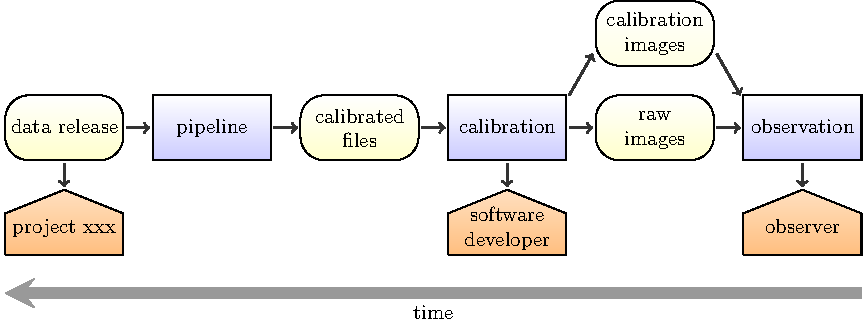
\includegraphics[width=1\textwidth]{workflow-backwards.pdf}
\caption[Example graph of provenance discovery]{An example graph of provenance discovery. Starting with a released dataset (left), the involved activities (blue boxes), 
progenitor entities (yellow rounded boxes) and responsible agents (orange pentagons) are 
discovered.}
\label{fig:example-workflow}
\end{figure}


\subsection{Goal of the provenance model}
\label{sec:goals}

The goal of this Provenance DM is to describe how provenance information arising from astronomy projects can be modelled, stored and exchanged. 
Its scope is mainly modelling of the flow of data, of the relations between pieces of data, and of processing steps. 
However, the Provenance DM is sufficiently abstract that its core pattern could be applied to any kind of process related to either observation or simulation data.

Information attached to observation activities such as ambient conditions and instrument characteristics provide useful information to assess the quality and reliability of the generated entities.
Contextual information during the execution of processing activities (computer structure, nodes, operating system used, etc.) can also be relevant for the description of the main entities generated. 
This complementary information should be included in the form of metadata or additional entities connected to an activity. 
However, the precise structure and modelling of this information is out of the scope of this document. 

In general, the model shall capture information in a machine-readable way that would enable a scientist who has no prior knowledge about a dataset to get more background information. 
This will help the scientist to decide if the dataset is adequate for her research goal, assess its quality and reliability and get enough information to be able to trace back its history as far as required or possible. 

Provenance information can be exposed with different granularity. A specific project has to decide this granularity.
The granularity and amount of provenance information provided depends on the available information, the needs of the project and the intended usage of this information.

This flexible approach has an impact on the interoperability between different services as this level of detail is not known a priori.
The objective of the model is to propose a general structure for the provenance information. In addition, proposed vocabularies of reserved words help to further formalize the detailed provenance information.


The following list is a collection of use cases addressed by the Provenance DM listed by goal categories.


\paragraphlb{A: Traceability of products}
        Track the lineage of a product back to the raw material (backwards search), show the
        workflow or the data flow that led to a product.

        \noindent Examples: 
        \begin{itemize}
            \item Having a dataset, find the main progenitors and in particular locate the raw data.
            \item Find out what processing steps have been already performed for a given dataset: Is an image already calibrated? What about dark field subtraction? Were foreground stars removed?
            \item Find out if a filter to remove atmospheric background muons has been applied.
        \end{itemize}


\paragraphlb{B: Acknowledgement and contact information}
        Find the people involved in the production of a dataset, the people\slash{}organizations\slash{}institutes that one may want to acknowledge or can be asked for more information.

        \noindent Examples: 
        \begin{itemize}
            \item I want to use an image for my own work -- who was involved in creating it? Who can I contact to get information? 
            \item Who was on shift while the data was taken?
            \item I have a question about column xxx in a data table. Who can I ask about that? 
        \end{itemize}


\paragraphlb{C: Quality and Reliability assessment}
Assess the quality and reliability of an observation, production step or dataset, e.g., based on detailed descriptions of the processing steps and manipulated entities.
        
        \noindent Examples:
        \begin{itemize}
            \item Get detailed information on the methods/tools/software that were involved: What algorithm was used for Cherenkov photon reconstruction? How was the stacking of images performed?
            \item Check if the processing steps (including data acquisition) went ``well'': Were there any warnings during the data processing? Any quality control parameters?
            \item Extract the ambient conditions during data acquisition (cloud coverage? wind? temperature?)
            \item Is the dataset produced or published by a person/organisation I trust? Using methods I trust?
        \end{itemize}


\paragraphlb{D: Identification of error location}
Find the location of possible error sources in the generation of a product. This is connected to use cases described in section C above, but implies an access to more information on the execution such as configuration or execution environment.

        \noindent Examples:
        \begin{itemize}
            \item I found something strange in an image. Was there anything strange noted when the image was taken? a warning during the processing? 
            \item Which pipeline version was used, the old one with a known bug for treating bright objects or a newer version? 
            \item What was the execution environment of the pipeline (operating system, system dependencies, software version, etc.)?
            \item What was the detailed configuration of the pipeline? were the parameters correctly set for the image cleaning step?
        \end{itemize}


\paragraphlb{E: Search in structured provenance metadata}
        Use Provenance criteria to locate datasets (forward search), e.g., finding all images produced by a certain processing step or derived from data which were taken by a given facility.
        
        \noindent Examples:
        \begin{itemize}
            \item Find more images that were produced using the same version of the CTA pipeline.
            \item Get an overview of all images reduced with the same calibration dataset.
            \item Are there any more images attributed to this observer?  
            \item Find all datasets generated using this given algorithm, with this given configuration, for this given step of the data processing.
            \item Find all generated data files that used incorrectly generated file X as an input, so that they can be marked for re-processing
            \item Extract all the provenance information of a SVOM light curve or spectrum to reprocess the raw data with refined parameters.
        \end{itemize}

\paragraphlb{General Remarks}
In addition to those use cases, if the stored information is sufficiently fine grained, it is possible to enable the \textbf{reproducibility} of an activity or sequence of activities, with the exact same configuration and exact same conditions.

Provenance information delivers additional information about a scientific dataset to enable the scientist to evaluate its \textbf{relevance for his work}.

\subsection{Requirements and best practices}
\label{sec:requirements}

\subsubsection{Model requirements}

This document was developed with these general requirements in mind:

\begin{itemize}

% == other models / serialisation

\item Provenance information MUST be formalized following a standard model, with corresponding standard serialization formats.

\item Provenance information MUST be machine readable.

\item Provenance data model classes and attributes SHOULD make use of existing IVOA standards.

\item Provenance information SHOULD be serializable into the W3C provenance standard formats (PROV-N, PROV-XML, PROV-JSON) with minimum information loss.

\item Entities, Activities and Agents MUST be uniquely identifiable within a domain.
% Provenance information can only be given for uniquely identifiable entities, at least inside their domain.
\end{itemize}


\subsubsection{Best practices}

The following additional points are recommended when managing provenance information within the VO context:

\begin{itemize}

% == links between entity/activity

\item The reliability of provenance information SHOULD be ensured (e.g. by an authority endorsing the information, or by provenance of provenance).

\item Provenance metadata for a given entity SHOULD contain information to find immediate progenitor(s).
%All produced entities must contain information to find its immediate progenitor(s).

\item An entity SHOULD be linked to the activity that generated it.
%Provenance metadata must contain information to find the activity that generated a given entity.
%* All produced entities must contain information to find the activity that generated it

\item Activities SHOULD be linked to input entities.
%(if applicable).

\item Activities SHOULD point to output entities.

\item Provenance information SHOULD make it possible to derive the logical sequence of activities.
%The order of the activities should be available.

%\item Provenance information should contain the list of activities and progenitor entities.
% too vague .... must be an ordered list ... One step should also be allowed.

%\item Released entities SHOULD have a main contact.
% same as below.

\item All activities and entities are recommended to have contact information and contain a (short) description or link to a description.
% could also be the documentation.

\end{itemize}


\subsection{Role within the VO Architecture}
\TODO{Will be inserted later.}
% Skipping this for now. Let's not let this draft look more official than it 
% currently is.

%\begin{figure}
%\centering
%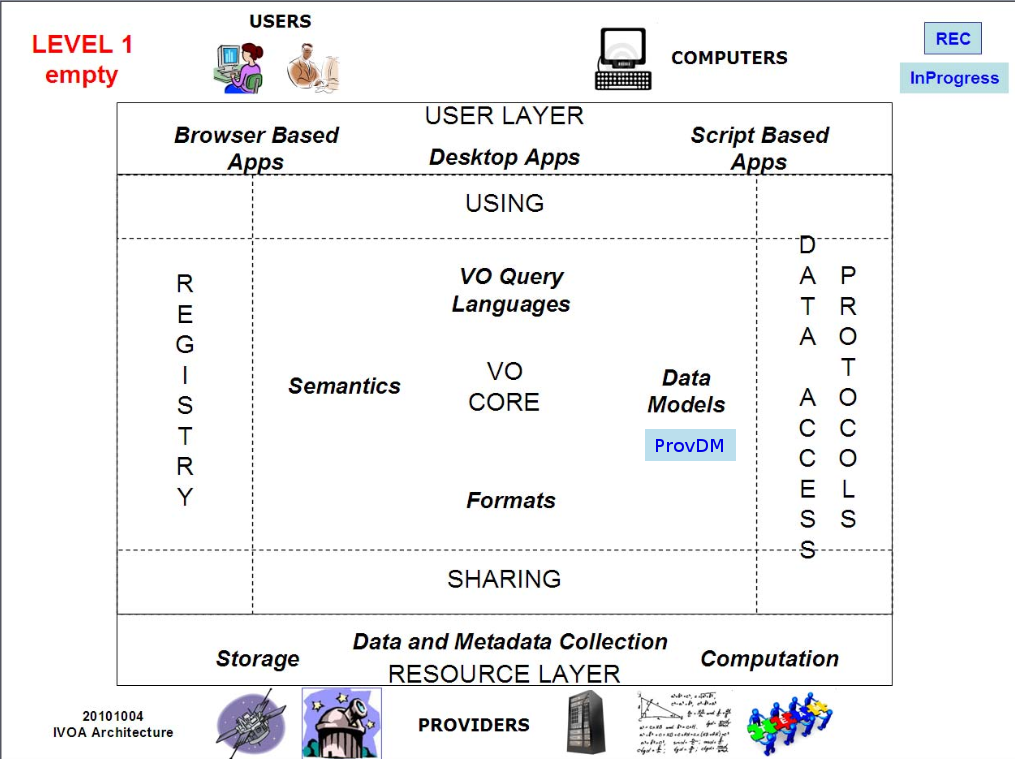
\includegraphics[width=0.9\textwidth]{archdiag.png}
%\caption{Architecture diagram for this document}
%\label{fig:archdiag}
%\end{figure}

%Fig.~\ref{fig:archdiag} shows the role this document plays within the
%IVOA architecture \citep{note:VOARCH}.

\subsection{Previous efforts}
The provenance concept was early introduced by the IVOA within the scope of the Observation Data Model (ref1 : IVOA note 2005) as a class describing where the data are coming from. A full observation data model dedicated to the specific spectral data was then designed (Ref2 : spectral data model) as well as a fully generic characterisation data model of the measureemnt axes of the data (ref3: characterisation data model) while the progress on the provenance data model were slowing down.

IVOA DM WG first gathered various use cases coming from different communities of observational  astronomy (optical,  radio, Xray, interferometry). Common motivations for a provenance tracing of the history included : quality assesment, discovery of dataset progenitors and access to metadata necessary for reprocessing. Provenance datamodel was then designed as the combination of Data processing, Observing Configuration and Observation ambiant conditions datamodel classes. 
The Processing class was embedding a sequence of processing stages which were hooking specific ad hoc details and links to input and output datasets, as well as processing step description. 
Despite the attempts of UML description of the model and writing of xml serialization examples the IVOA effort failed to provide a workable solution:  the scope was probably too ambitious and the technical background too instable. A compilation of these early developments can be found on the IVOA site (ref4). From 2013 onwards IVOA concentrated on use cases related to processing description and decided to design the model  by extending the basic W3C provenance basic structure,as described in the current specification. 

Outside of the astronomical community, the Provenance Challenge series (2006 -- 2010), a community effort to achieve inter-operability between different representations of provenance in scientific workflows, resulted in the Open Provenance Model (\cite{moreau2010}). 
Later, the W3C Provenance Working Group was founded and released the W3C Provenance Data Model as Recommendation in 2013 (\cite{std:W3CProvDM}). 
OPM was designed to be applicable to anything, scientific data as well as cars or immaterial things like decisions. With the W3C model, this becomes more focused on the web.  Nevertheless, the core concepts are still in principle the same in both models and very general, so they can be applied to astronomical datasets and workflows as well. 
The W3C model was taken up by a larger number of applications and tools than OPM, we are therefore basing our modeling efforts on the W3C Provenance data model, making it less abstract and more specific, or extending it where necessary. 


The W3C model even already specifies PROV-DM Extensibility points (section 6 in \cite{std:W3CProvDM}) for extending the core model. This allows one to specify additional roles and types to each entity, agent or relation using the attributes \texttt{prov:type} and \texttt{prov:role}.
By specifying the allowed values for the IVOA model, we can adjust the model to our needs while still being compliant to W3C.




\section{The provenance data model}
% updates Mireille  2017 April/May 2nd 
%roles for Agents -updates  + funder
% 
In this section, we describe the currently discussed Provenance Data Model. We 
start with an UML class diagram, explain the core elements and then give 
in the following sections more details for each class and relation.
An auto-generated documentation of all classes (VO-DML compliant) is available in the Volute repository at \url{https://volute.g-vo.org/svn/trunk/projects/dm/provenance/vo-dml/ProvenanceDM.html}.

\subsection{Overview: Conceptional UML class diagram and introduction to core classes}
%We give in this section an overview on the main classes. More details about 
%each class and their relations will be explained in the following sections.
%Its core elements are colored in blue. These core elements can also be found in the W3C Provenance Data
%Model. The pattern defined by these classes is very general and can be reused everywhere where provenance is needed. 

\begin{figure}[h]
\centering
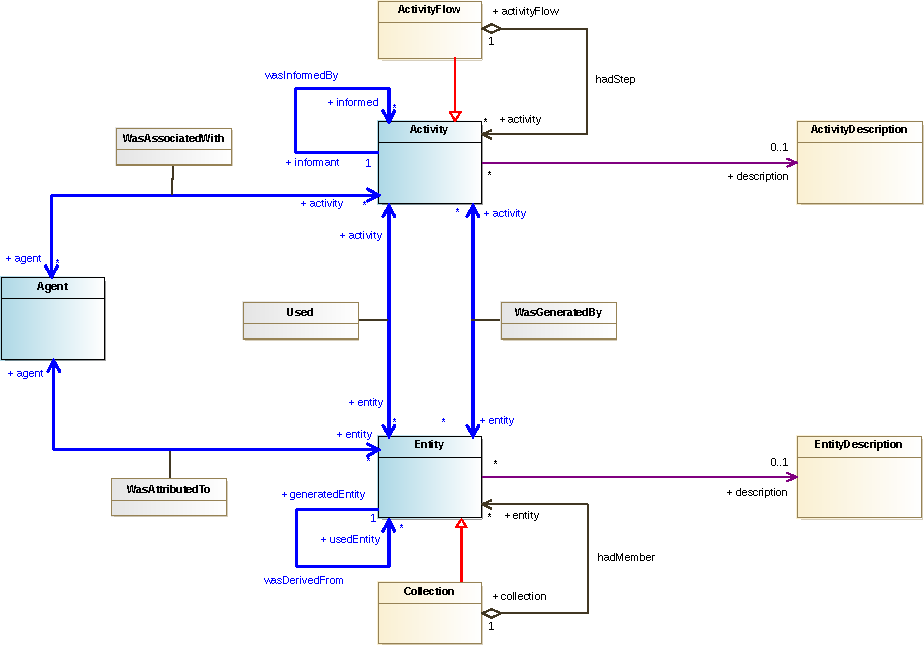
\includegraphics[width=1.0\textwidth]{../datamodel-diagrams/images/domain-classdiagram-v2.pdf}
\caption{Overview of the classes for the Provenance Data Model in a conceptual class diagram. The blue classes are core elements. There appear a number of many-to-many relationships with attached association classes (grey) which can contain additional attributes.}
%Objects in the blue box also appear in the W3C Provenance Data Model. 
%Green classes are links to the IVOA Dataset Metadata Model.}
\label{fig:classdiagram-conceptional}
\end{figure}


%\label{sec:core}
% Some examples for different use cases are given in Section \ref{sec:usecases-implementations}.
% The elements of a provenance model can be expressed as a directed graph to capture the causal dependencies. 

Figure~\ref{fig:classdiagram-conceptional} shows the conceptional UML diagram for an IVOA Provenance Data
Model.
The core elements of the Provenance Data Model are \class{Entity}, \class{Activity} and \class{Agent}. 
We chose for these elements the same names as were used in the Provenance Data 
Model of the World Wide Web Consortium (W3C, \citealt{std:W3CProvDM}), which defines 
a very abstract pattern that can be reused here. Here are the core classes with 
a short description and some examples:

\begin{itemize}
\item \class{Entity:} a thing at a certain state\\
    examples: data products like images, catalogs, parameter files, calibration data, instrument characteristics

\item \class{Activity:} an action/process or a series of actions, occurs over a period of time, performed on or caused by entities, usually results in new entities\\
    examples: data acquisition like observation, simulation; regridding, fusion, calibration steps, reconstruction

\item \class{Agent:} executes/controls an activity, is responsible for an activity or an entity\\
    examples: telescope astronomer, pipeline operator, principal investigator, software engineer, project helpdesk

\end{itemize}

\noindent



\begin{figure}[h]
\centering
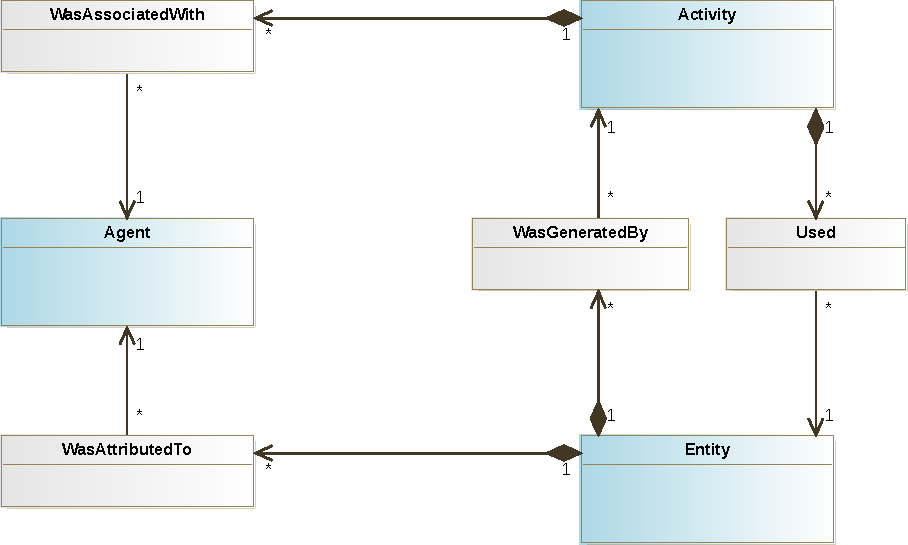
\includegraphics[scale=0.6]{../datamodel-diagrams/images/classes-core-w3c.pdf}
\caption{The main core classes and relations of the Provenance Data Model, which also occur in the W3C model.}
\label{fig:coreclasses}
\end{figure}

These core classes along with their relations to each other are provided in Figure~\ref{fig:coreclasses}.
We use the following relation classes to specify the mapping between the three core 
classes. 
The relation names were again chosen to match the W3C model names:
\begin{itemize}
\item \class{WasGeneratedBy:} a new entity is generated by an activity\\
        (entity ``image m31.fits'' wasGeneratedBy activity ``observation'')
\item \class{Used:} an entity is used by an activity\\
        (activity ``calibration'' used entities ``calibration data'', ``raw images'')
\item \class{WasAssociatedWith:} agents have responsibility for an activity\\
        (agent ``observer Max Smith'' wasAssociatedWith activity ``observation'')
\item \class{WasAttributedTo:} an entity can be attributed to an agent\\
        (entity ``image m31.fits'' wasAttributedTo ``M31 observation campaign'')
\end{itemize}

Note that the relations appear as extra classes (and thus boxes in the diagrams, instead of just having annotated relations), because they can have additional attributes -- when mapping the model to a relational database, these relations would appear as mapping tables.

In the domain of astronomy, certain processes and steps are repeated again and 
again with different parameters. We therefore separate the descriptions of activities
from the actual processes and introduce an additional \class{ActivityDescription} class (see Figure~\ref{fig:classdiagram-conceptional}).
Likewise, we also apply the same pattern for \class{Entity} and add an \class{EntityDescription}
class.
Defining such descriptions allows them to be reused, which is very useful 
when performing a series of tasks of the same type, as is typically done in 
astronomy. 

A similar normalization of descriptions of the actual processes and datasets 
can also be found in the IVOA Simulation Data Model \citep[SimDM, ][]{std:SimDM}), 
which describes simulation metadata. The SimDM classes \class{Experiment} and \class{Protocol} 
correspond to the Provenance terms \class{Activity} and \class{ActivityDescription}.

%The W3C-model has the advantage of being already an approved standard, and it 
%contains all the necessary main features needed for a Provenance model for 
%Astronomy. However, it is very general, and by adding reusable prototypes, 
%templates or descriptions for activities and entities,  the model may fit better 
%to the astronomy domain.

This separation into two classes may not be needed for each and every project,
and everyone is free to choose which classes make sense for his/her use case.
When serializing provenance, one can integrate the description side into the 
other classes, thus producing a W3C compliant provenance description. More details about 
all these classes and relations are given in the following section.


%It still remains to be seen if this separation into two classes is necessary, 
%useful or just nice to have. Currently, we include the descriptions in our model, 
%for normalization purposes. 

%But when serialising the provenance one could 
%integrate the description side into the other classes, thus producing W3C 
%compliant provenance.


\subsection{Model description}

\subsubsection{Class diagram and VO-DML compatibility}
\begin{figure}[h]
\centering
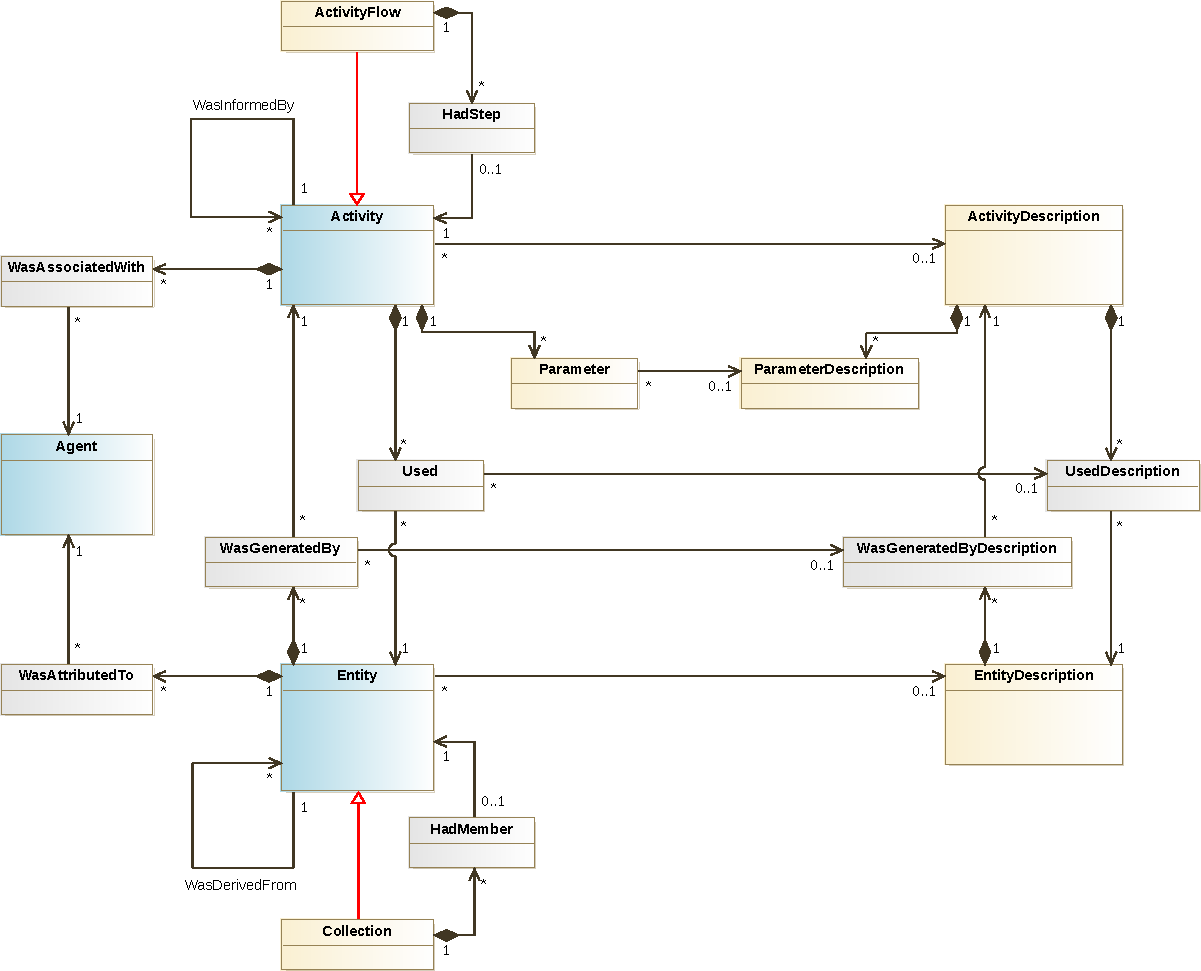
\includegraphics[width=1.0\textwidth]{../datamodel-diagrams/images/classes-overview.pdf}
\caption{More detailed overview of the classes for the Provenance Data Model. Note that this UML class diagram is more compatible with VO-DML.}
\label{fig:classdiagram}
\end{figure}

Figure~\ref{fig:classdiagram} shows the full class diagram with the association classes for the many-to-many relations modeled more directly as mapping classes. When implementing the model in a relational database, these classes can be represented as individual tables for mapping the relation. We model one of the associations of the many-to-many relationships as composition (full diamond), if the mapping class belongs more strongly to one of its linked classes, e.g. the \emph{Used} relations are strongly dependent on the corresponding \emph{Activities}. The documentation of all classes and an automatically generated figure based on the underlying xmi-description behind this UML diagram is available in the Volute repository at
\url{https://volute.g-vo.org/svn/trunk/projects/dm/provenance/vo-dml/ProvenanceDM.html}.

This version of the UML diagram is fully VO-DML compliant, i.e. we just used the restricted subset of UML to model
Provenance and reused the IVOA datatypes.


\subsubsection{Entity and EntityDescription}

Entities in astronomy are usually astronomical or astrophysical datasets in the 
form of images, tables, numbers, etc. But they can also be observation or 
simulation log files, files containing system information, environment variables, names and versions of packages, ambient conditions or, in a wider sense, also observation proposals, scientific 
articles, or manuals and other documents. 

An entity is not restricted to being a file. 
It can even be just a number in a table, depending on how fine-grained the 
provenance shall be described.

\begin{figure}[h]
\centering
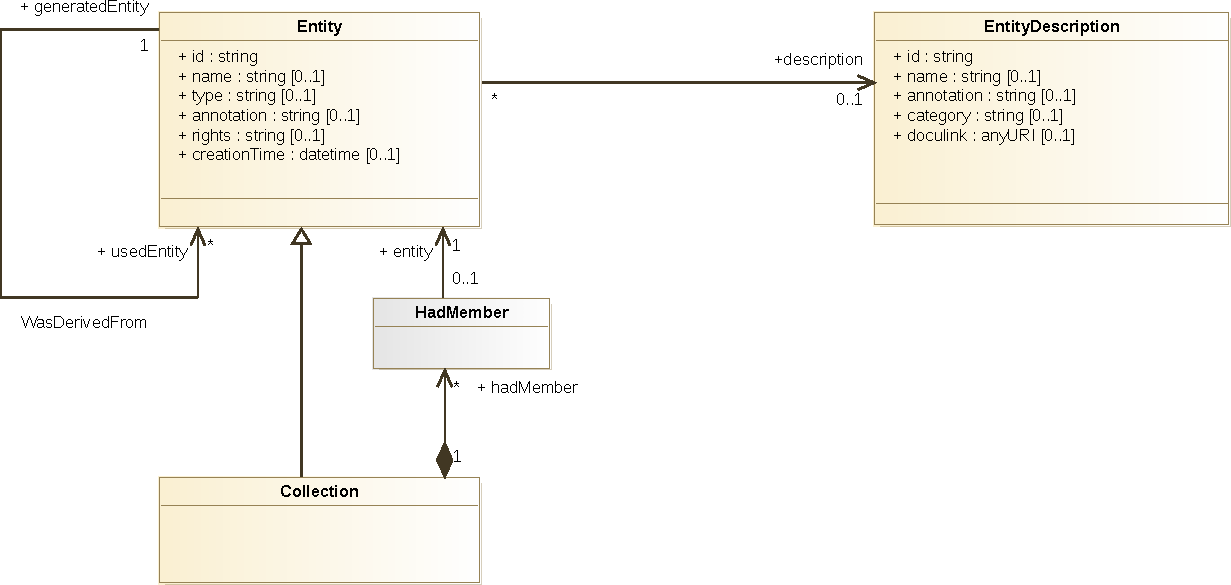
\includegraphics[scale=0.6]{../datamodel-diagrams/images/entity-details-v2.pdf}
\caption{The relation between Entity, EntityDescription and Collection (see Section~\ref{sec:collection}). 
Links to the Dataset class from the Dataset Metadata Model are described in Section~\ref{sec:dmlinks}.}
\label{fig:entity-details}
\end{figure}

The VO concept closest to Entity is the notion of ``Dataset'', which could mean a single 
table, an image or a collection of them. The Dataset Metadata Model 
\citep{std:DatasetDM} specifies an ``IVOA Dataset'' as ``a file or files which 
are considered to be a single deliverable''. 
Most attributes of the \class{Dataset} class can be mapped
directly to attributes of the \class{Entity} and EntityDescription class, see the mapping table \ref{tab:datasetmapping} in Section~\ref{sec:dmlinks}.


\begin{table}[h]

\small
\tymax  0.5\textwidth

\textbf{\normalsize Entity}\vspace{0.25em}\\
\begin{tabulary}{1.0\textwidth}{@{}lp{3.5cm}p{2cm}L@{}}
\toprule
\head{Attribute} & \head{W3C ProvDM} & \head{Data type} & \head{Description}\\
\midrule
\textbf{id} & prov:id & (qualified) string & a unique id for this entity (unique in its realm)\\
name       & prov:label & string & a human-readable name for the entity (to be displayed by clients)\\
type        & prov:type  & string & a provenance type, i.e. one of: prov:collection, prov:bundle, prov:plan, prov:entity; not needed for a simple entity\\
%description\_ref  & & foreign key/url & link to \class{EntityDescription}\\
annotation  & prov:description & string & text describing the entity in more detail\\
rights      & -- & string & access rights for the data, values: public, restricted or internal; can be linked to Curation.Rights from ObsCore/Dataset Metadata Model\\
creationTime  & -- & datetime & date and time at which the entity was created (e.g. timestamp of a file)\\
\midrule
\multicolumn{4}{l}{\textbf{Additional attributes:}} \\
\multicolumn{4}{l}{Further project specific attributes (e.g. size, path, url, \dots) can be added }\\
\multicolumn{4}{l}{(see Section \ref{sec:dataset-obscore})}\\
\bottomrule
\end{tabulary}
\caption{Attributes of entities. Mandatory attributes are marked in bold.
}\label{tab:entity-attributes}
\end{table}

For entities, we suggest the attributes given in Table 
\ref{tab:entity-attributes}. If the attribute also exists in the W3C 
Provenance Data Model, we list its name in the second column.

%We discussed further attributes like \emph{size} and \emph{format}, but we decided to treat an
%entity of the same content but different format (and thus size) as the same entity,
%unless they do not have the same provenance (e.g. when the ``transformation'' activity
%for converting one format into another is included in the provenance description).

%\TODO{format and size may not be needed, if entities with the same content but different format and size are considered as the same entity.}

The difference between entities that are used as input data or output data 
becomes clear by specifying the relations between the data and activities producing or using these data.
More details on this will follow in Section \ref{sec:entity-activity-relations}.

\paragraph{EntityDescription.}
%The Entity class can have an EntityDescription class attached. 
The types of entities, or datasets in astronomy, can be predefined using a description class \class{EntityDescription}.
This class is meant to store descriptive informations about an Entity that are known before the Entity instance is created. For example, if we run an activity to create a RGB image from three grey images, we may have a mandatory ``format'' for the input and output images before the execution (JPG, PNG, FITS\dots), but we probably cannot know the final ``size'' of the image  that will be created. Therefore, ``format'' would be an EntityDescription attribute , while ``size'' would be an attribute of the Entity instance. 

%This class thus stores entity-related 
Additional attributes that describe the content of the data could be derived from 
the Dataset Metadata Model (see Section \ref{sec:dataset-obscore})

The \class{EntityDescription} does NOT contain any information about the usage 
of the data, it tells nothing about them being used as input or output. This is 
defined only by the relations (and the relation descriptions) between activities
and entities (see Section \ref{sec:entity-activity-relations}).

The EntityDescription general attributes are summarized in Table 
\ref{tab:entitydescription-attributes}.


\begin{table}[h]
\small
\tymax  0.5\textwidth
\textbf{\normalsize EntityDescription}\vspace{0.25em}\\
\begin{tabulary}{\textwidth}{@{}p{2.75cm}p{0cm}p{2cm}L@{}}
\toprule
\head{Attribute} & \head{} & \head{Data type} & \head{Description}\\
\midrule
\textbf{id} & & (qualified) string & a unique identifier for this description\\
name       & & string & a human-readable name for the entity description\\
annotation  & & string & a decriptive text for this kind of entity\\
category    & & string & specifies if the entity contains information on logging, system (environment), calibration, simulation, observation, configuration, ...\\
doculink    & & url & link to more documentation\\
% removed the obscore attributes, since specific for observations only, not applicable to configuration entities etc.
% dataproduct\_ type  & & string       & from ObsCore data model \citep{std:ObsCore}, if applicable; describes, what kind of product it is (e.g. image, table)\\
% dataproduct\_ subtype & & string       & from ObsCore data model, more specific subtype\\
% level       & & enum integer & the level of processing or calibration; for ObsCore's calib\_level it is an integer between 0 and 3\\
\midrule
\multicolumn{4}{l}{\textbf{Additional attributes:}} \\
\multicolumn{4}{l}{\emph{Further project specific attributes (e.g.} format, content\_type, dataproduct\_type \emph{and} }\\
\multicolumn{4}{l}{\_subtype, version, calibLevel, \dots) \emph{can be added, maybe related to the DatasetDM }}\\
\multicolumn{4}{l}{(Section \ref{sec:dataset-obscore})}\\
\bottomrule
\end{tabulary}
\caption{Attributes of \class{EntityDescription}. For simple use cases, 
this description class may be ignored and its attributes may be used for 
\class{Entity} instead.
%The utypes may vary depending on the data model, e.g. for simulation data they 
%would point to utypes of SimDM.
}\label{tab:entitydescription-attributes}
\end{table}


\begin{table}[h]

\small
\tymax  0.5\textwidth

\textbf{\normalsize WasDerivedFrom}\vspace{0.25em}\\
\begin{tabulary}{1.0\textwidth}{@{}lp{3cm}L@{}}
\toprule
\head{Attribute} & \head{Data type}   & \head{Description}\\
\midrule
id               & string              & a unique id for this entity (unique in its realm)\\
\textbf{generatedEntity} & string      & foreign key to the entity\\
\textbf{usedEntity}      & string      & foreign key to the progenitor, from which the generatedEntity was derived\\
activity         & string              & foreign key to the generation activity\\
generation       & string              & foreign key to the wasGeneratedBy relation\\
usage            & string              & foreign key to the used relation\\
\bottomrule
\end{tabulary}
\caption{Attributes of the WasDerivedFrom relation. This is the same as used in W3C's ProvDM. Mandatory attributes are marked in bold.
}\label{tab:wasderivedfrom-attributes}
\end{table}


\paragraph{WasDerivedFrom.}
In Figure~\ref{fig:entity-details} there is one more relation that we have not mentioned yet: 
the \class{WasDerivedFrom}-relation which links two entities together, borrowed from the W3C model. 
It is used to express that 
one entity was derived from another, i.e. it can be used to find one (or more) progenitor(s) 
of a dataset, without having to look for the activities in between. It can therefore serve as 
a shortcut.

The information this relation provides is somewhat redundant, since progenitors for entities
can be found through the links to activity and the corresponding descriptions.
Nevertheless, we include \class{WasDerivedFrom} for those cases where an explicit 
link between an entity and its progenitor is useful (e.g. for speeding up searches for 
progenitors or if the activity in between is not important).

Note that the \class{WasDerivedFrom} relation
cannot always automatically be infered from following \class{WasGeneratedBy} and \class{Used} relations alone:
If there is more than one input and more than one output of an activity, it is not clear (without 
consulting the activityDescription and entity roles in the relation-descriptions) which entity was derived from which.
Only by specifying the descriptions and roles accordingly or by adding the a \class{WasDerivedFrom} relation,
this direct derivation becomes known.



\subsubsection{Collection}\label{sec:collection}
Collections are entities that are grouped together and can be treated as one single entity. 
From the provenance point of view, they have to have the \emph{same origin}, i.e., they were 
produced by the same activity (which could also be the activity of collecting
data for a publication or similar). The term ``collection'' is 
also used in the Dataset Metadata Model for grouping datasets.
% (but with a slightly different meaning). 
As an example, a collection 
with the name `RAVE survey' could consist of a number of database tables and spectra files.

%\TODO{Do we allow empty collections? Or should collections always contain at least 1 member? (otherwise they are just prov:entities?)}

The Entity-Collection relation can be modeled using the \emph{Composite} design pattern: 
Collection is a subclass of Entity, but also an aggregation of 1 to many entities, 
which could be collections themselves. 
In order to be compliant to VO-DML, we model the membership-relation explicitly 
by including a \class{HadMember} class in our model, which is connected to the
\emph{Collection} class via a composition. It may contain an additional role attribute.

Collections are also known in the W3C model, in the same sense as used here.
The relation between entity and collection is also called ``HadMember'' in the W3C model.

An additional class \class{CollectionDescription} is only 
needed if it has different attributes than 
the \class{EntityDescription}. This class should therefore only be introduced if a use case requires it.

\paragraph{Advantages of collections:} Collections can be used to collect entities with the same provenance information together, 
    in order to hide complexity where necessary. They can be used for defining 
    different levels of detail (granularity).

%\TODO{Find a really strong use case for Collections to convince everyone that they are useful/needed.}

\subsubsection{Activity and ActivityDescription}
\label{sec:activity}

\begin{figure}[h]
\centering
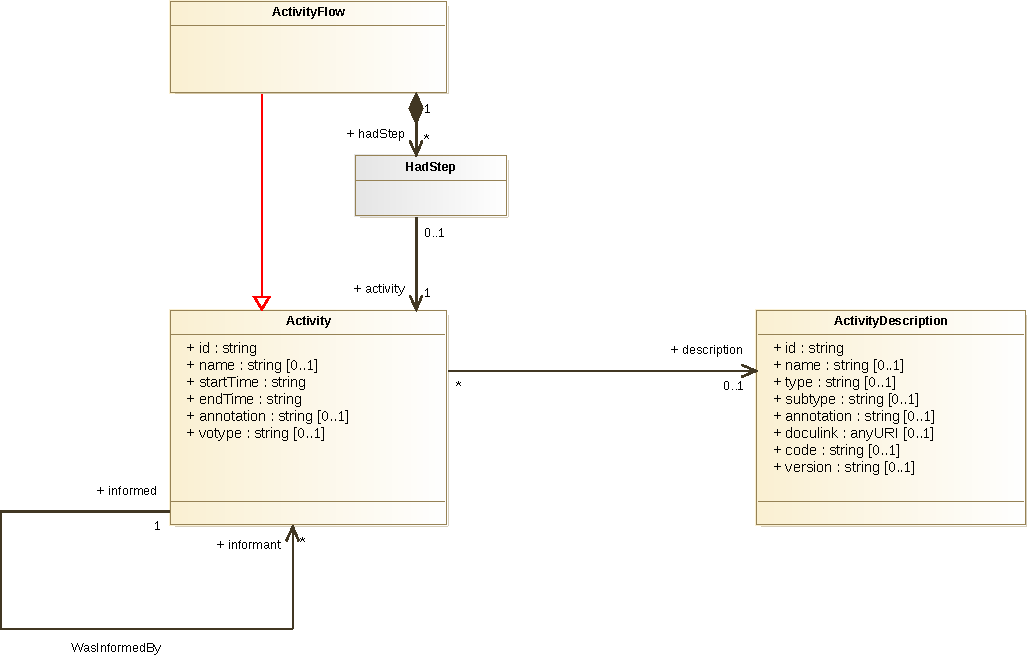
\includegraphics[scale=0.5]{../datamodel-diagrams/images/activity-details.pdf}
\caption{Details for Activity, ActivityDescription and ActivityFlow (see Section~\ref{sec:activityflow}). 
}
\label{fig:activity-details}
\end{figure}

\begin{table}[h]

\small
\tymax  0.5\textwidth

\textbf{\normalsize Activity}\vspace{0.25em}\\
\begin{tabulary}{1.0\textwidth}{@{}lp{2.5cm}p{2cm}L@{}}
\toprule
\head{Attribute} & \head{W3C ProvDM} & \head{Data type} & \head{Description}\\
\midrule
\textbf{id} & prov:id  & (qualified) string & a unique id for this activity (unique in its realm)\\
name        & prov:label  & string & a human-readable name (to be displayed by clients)\\
\textbf{startTime} & prov:startTime & datetime & start of an activity\\
\textbf{endTime} & prov:endTime  & datetime & end of an activity\\
annotation        & prov:description & string & additional explanations for the specific activity instance\\
%description\_ref  &  & foreign key/url & link to \class{ActivityDescription}\\
\bottomrule
\end{tabulary}
\caption{Attributes of \class{Activity}, their data types and equivalents in the W3C Provenance 
Data Model, if existing. Attributes in bold are \textbf{mandatory}.}
\end{table}


\begin{table}[ht]
\small
\tymax  0.5\textwidth
\textbf{\normalsize ActivityDescription}\vspace{0.25em}\\
\begin{tabulary}{1.0\textwidth}{@{}p{0cm}p{2.5cm}lL@{}}
\toprule
\head{Attribute} & \head{} & \head{Data type} & \head{Description}\\
\midrule
\textbf{id}  & & string & a unique id for this activity description (unique in its realm)\\
name         & & string & a human-readable name (to be displayed by clients)\\
type         & & string & type of the activity, from a vocabulary or list, e.g. data acquisition (observation or simulation), reduction, calibration, publication\\
subtype      & & string & more specific subtype of the activity\\
annotation  & & string & additional free text description for the activity\\
%code         & & string & the code used for this process\\
%version      & & string & a version number for the code\\
doculink     & & url    & link to further documentation on this process, e.g. a 
paper, the source code in a version control system etc.\\
\bottomrule
\end{tabulary}
\caption{Attributes of \class{ActivityDescription}.}
\end{table}


Activities in astronomy include all steps from obtaining data to the reduction of 
images and production of new datasets, like image calibration, bias subtraction, image stacking; 
light curve generation from a number of observations, radial velocity 
determination from spectra, post-processing steps of simulations etc.

\paragraph{ActivityDescription.}
The method underlying an activity can be specified by a corresponding 
\class{ActivityDescription} class (previously named \class{Method}, corresponds 
to the \class{Protocol} class in SimDM). This could be, 
for instance, the name of the code used to perform an activity or a more general 
description of the underlying algorithm or process. An activity is then a 
concrete case (instance) of using such a method, with a startTime and endTime, 
and it refers to a corresponding description for further information.

There MUST be exactly zero or one \class{ActivityDescription} per \class{Activity}. If steps from a 
pipeline shall be grouped together, one needs to create a proper 
\class{ActivityDescription} for describing all the steps at once. This method can then 
be refered to by the pipeline-activity. 

When serializing the data model, the attributes
of the description class may be assigned to the activity in order to produce 
a W3C compliant serialization (same as with Entity/EntityDescription).


\paragraph{WasInformedBy.}
The individual steps of a pipeline can be chained
together directly, without mentioning the intermediate datasets, using the \class{WasInformedBy}-relation.
This relation can be used as a short-cut, if the exchanged datasets are deemed to be not important
enough to be recorded. For grouping activities, also see the 
next section \ref{sec:activityflow}.


\subsubsection{ActivityFlow}\label{sec:activityflow}
%\TODO{Link to D-PROV!}
For facilitating grouping of activities (and their related entities etc.)
we introduce the class \class{ActivityFlow}.
It can be used for hiding and grouping a part of the workflow/pipeline 
or provenance 
description, if different levels of granularity are needed. Such pipelines and workflows are very common in astronomical data production and processing. Figure \ref{fig:provgraph-activityflow}
illustrates an example provenance graph in a detailed level (left side) 
and using the ActivityFlow (right side).


\begin{figure}[h]
\centering
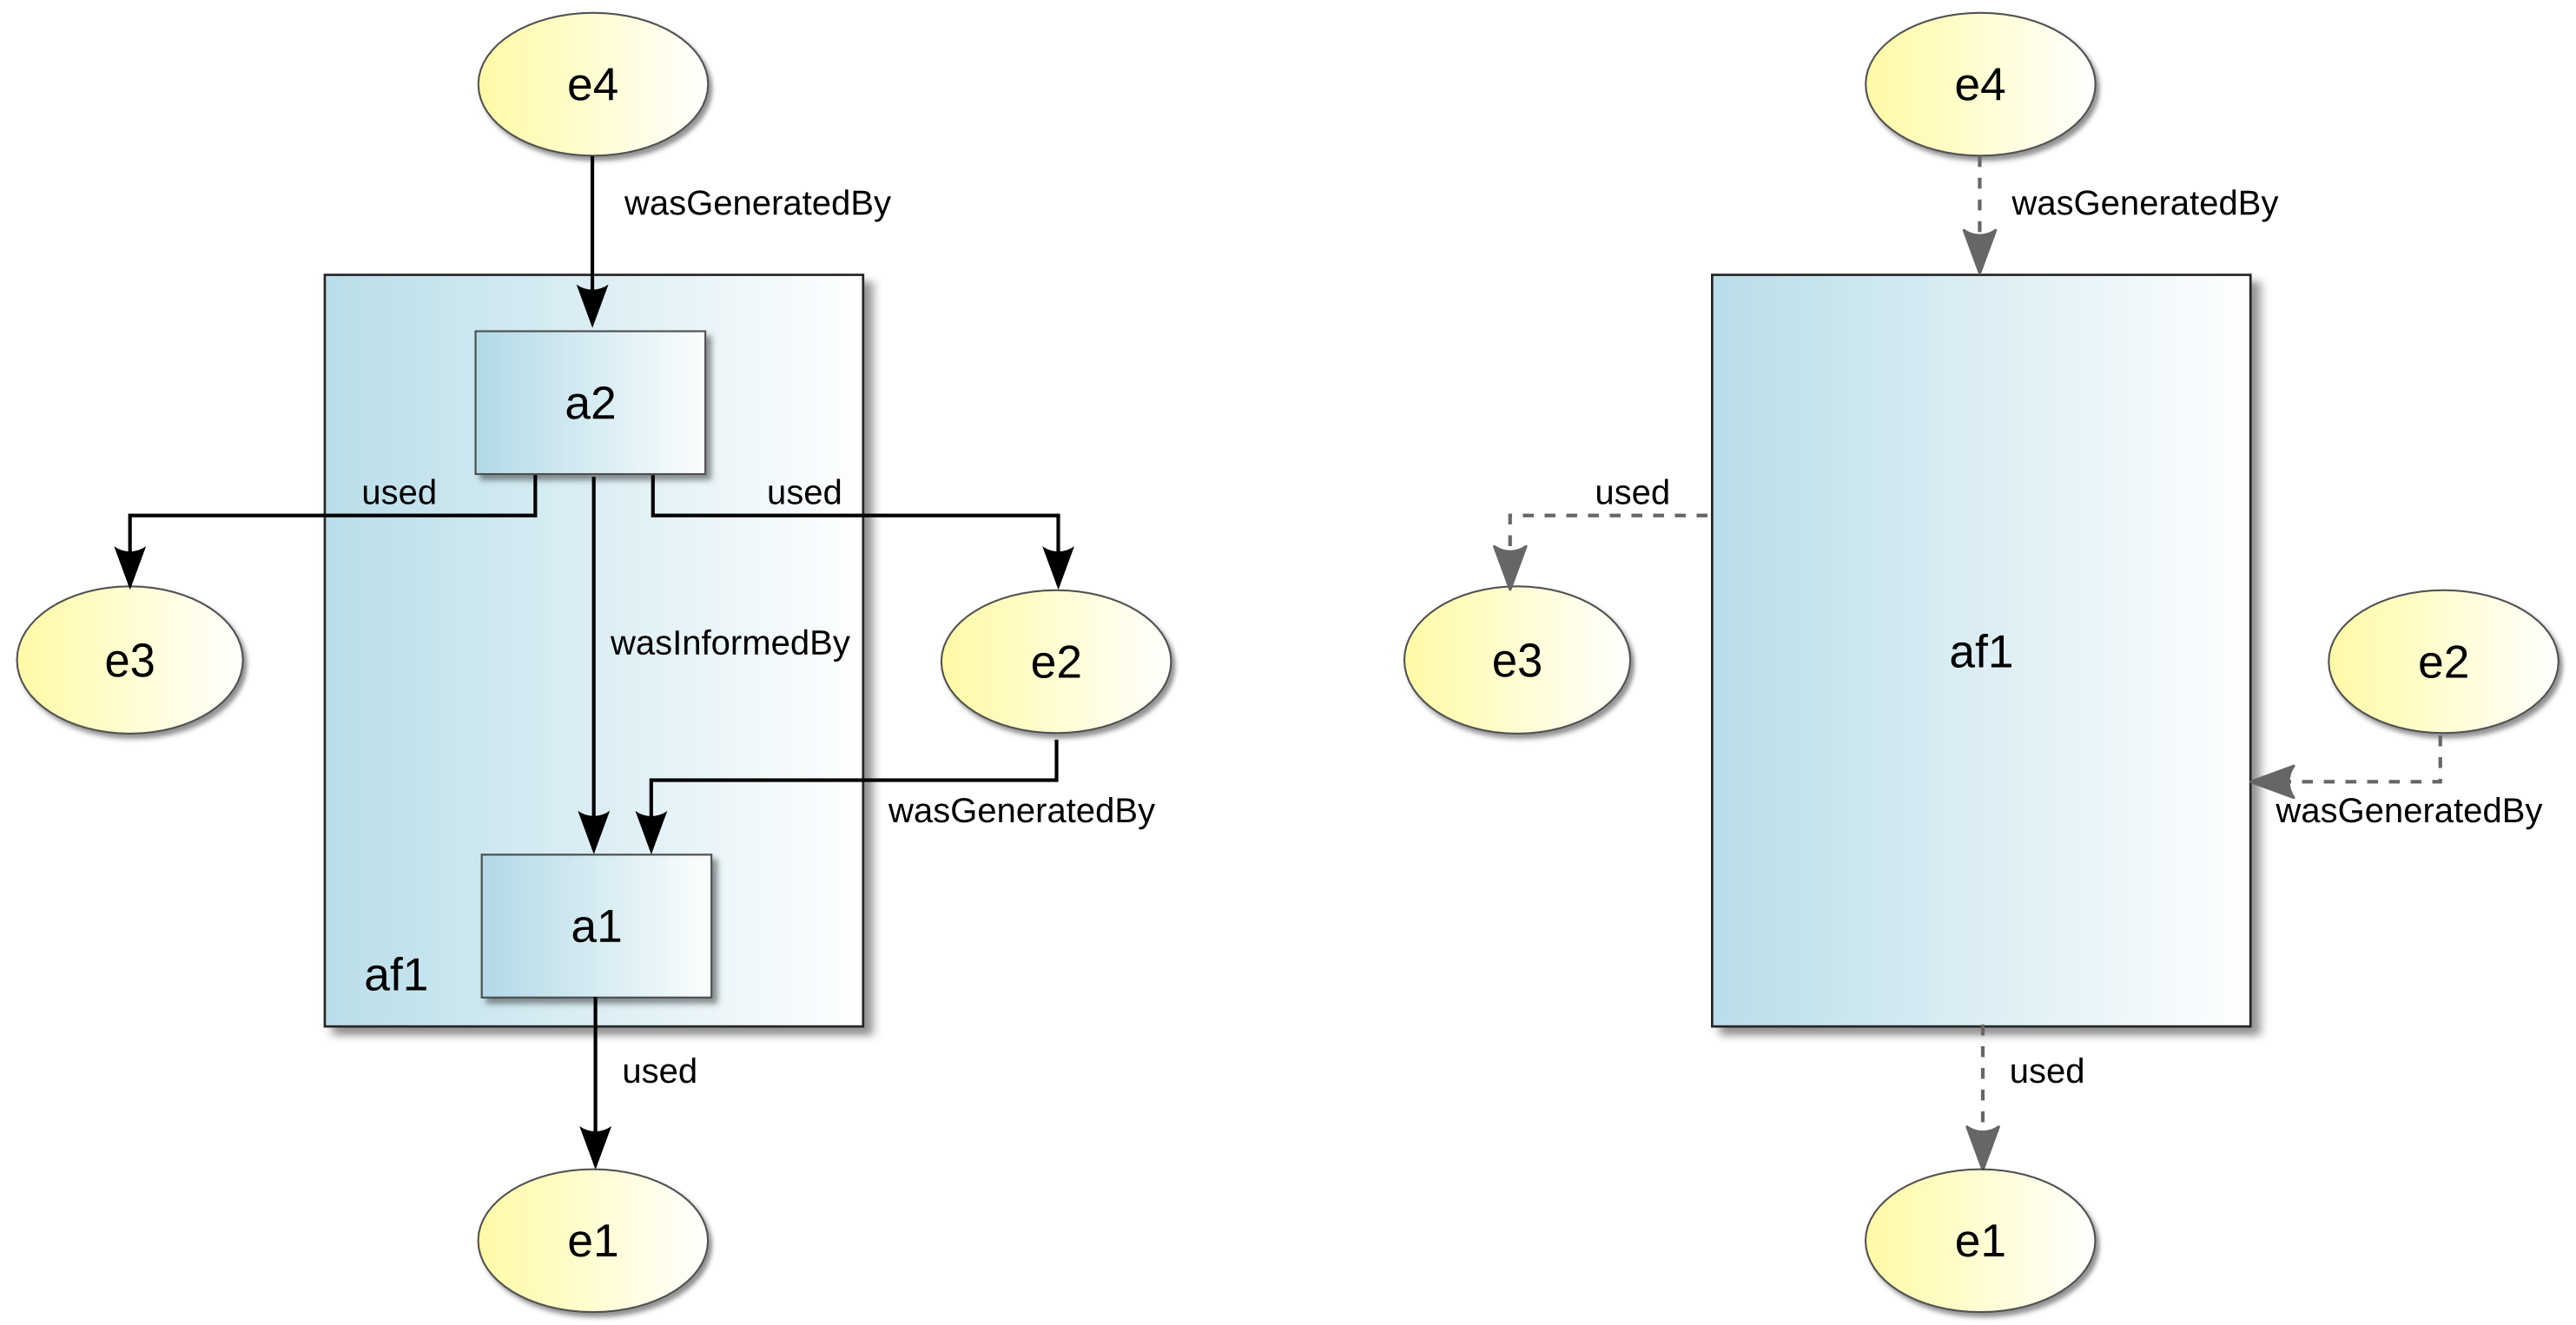
\includegraphics[width=1\textwidth]{../datamodel-diagrams/images/provgraph-activityflow}
\caption{An example provenance graph. The detailed version is shown on the left side. It also shows
the shortcut \class{WasInformedBy} to connect two activities, which could be used if the entity e2 
would not be needed anywhere else.
An ActivityFlow can be used to ``hide'' a part of the provenance graph as is shown on the right side.
Activities are marked by blue rectangles, entities by yellow ellipses.}
\label{fig:provgraph-activityflow}
\end{figure}

We also explored the different ways to describe a set of activities in the W3C 
provenance model. This model uses \class{Bundle}, i.e. an entity with type ``Bundle'', 
for wrapping a provenance description. Each part of a provenance description can be 
put into a bundle, and the bundle can then be reused in other provenance descriptions. 
W3C's \class{Plan} is an entity with type ``Plan'' and is used for describing a 
set of actions or steps. Both, \class{Bundle} and \class{Plan}, are entities and 
have the attributes and relations of this class (and thus one can define provenance of bundles and plans as well).

But we would like to consider a set of activities as being an \class{Activity} itself, 
with all the relations and properties that an activity also has. Therefore we do not reuse
W3C's classes for describing workflows and plans, but added 
the class \class{ActivityFlow} as an activity composed of activities. The composition is represented by 
the ``hadStep'' relation, as is shown in Figure~\ref{fig:activity-details}.

%while still making it obvious that this 
%group contains activities, we introduce the class \class{ActivityFlow}.
%This can be used for describing workflows or pipelines, or for 
%
%We also allow ActivityCollections to consist of a whole provenance graph of 
%activities and entities being linked together.


%We could introduce an additional abstract class, e.g. \class{AbstractActivity}, with \class{Activity} and 
%\class{ActivityFlow} being subclasses to this one. But this adds another layer of complexity 
%that we may not want in this data model.

%Since we introduced \class{ActivityFlow} mainly for having different view levels, 
%we may want to add an attribute \emph{viewLevel} to descriptions of activityflows.
% But where to set the 0 point for viewLevel???

\begin{figure}[h]
\centering
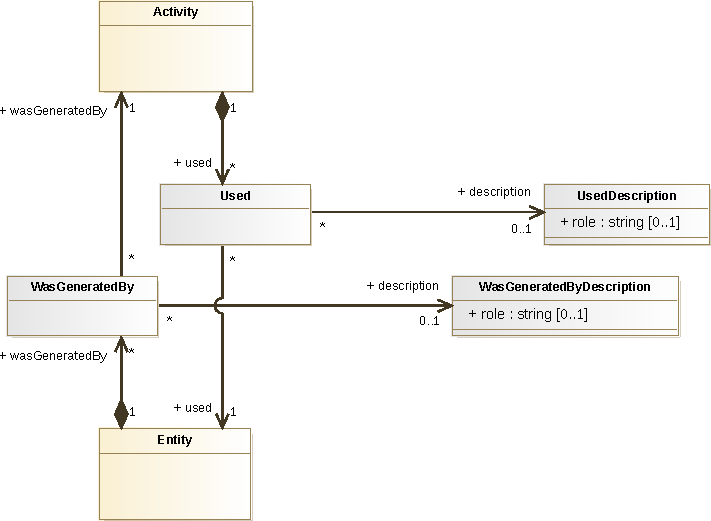
\includegraphics[scale=0.6]{../datamodel-diagrams/images/entity-activity-relations.pdf}
\hspace{0.15\textwidth}
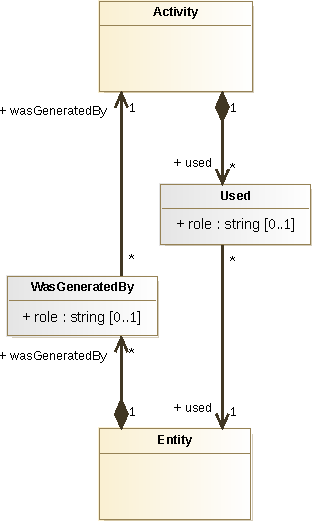
\includegraphics[scale=0.6]{../datamodel-diagrams/images/entity-activity-relations-nodesc.pdf}
\caption{\class{Entity} and \class{Activity} are linked via the \class{Used} and \class{WasGeneratedBy} relations. In the left image, the \emph{role} that an entity which was used or generated by an activity played is recorded with the corresponding \emph{UsedDescription} and \emph{WasGeneratedByDescription}, also see Section~\ref{sec:entity-roles}. If these description classes are not used, the \emph{role} can be used directly as an attribute within the \emph{Used} and \emph{WasGeneratedBy} classes (right image).}
\label{fig:entity-activity-relations}
\end{figure}


\subsubsection{Entity-Activity relations}\label{sec:entity-activity-relations}

For each data flow it should be possible to clearly identify entities and 
activities. 
%If the activities shall not be recorded explicitely, one could also 
%use the \emph{Derivation}-relation as suggested in the W3C Provenance Data Model
%to link derived entities to their originals.
Each entity is usually a result from an activity, expressed by a link from 
the entity to its generating activity using the \class{WasGeneratedBy} relation,
and can be used as input for (many) other activities, expressed by the \class{Used} relation.
Thus the information on whether data is used as input or was produced as output of 
some activity is given by the \emph{relation-types} between activities and entities.
%In fact, 
%it would be enough to provide this information just for the relations on the description side (right).
% -- Is this true?

We use two relations, \class{Used} and \class{WasGeneratedBy}, instead of just one
mapping class with a flag for input/output, because their descriptions and role-attributes
can be different. 
%in order to model the different 
%multiplicities explicitely: an entity always has only one (or none) 
%\class{WasGeneratedBy} relation, but may be \class{Used} many times as input for 
%different activities.

The \class{WasGeneratedBy}-relation can have the optional attribute \emph{time} -- this is the time, when 
the generation of the entity is finished. This generation time corresponds to e.g. \emph{DataID.date} in 
Dataset Metadata DM.
%It therefore corresponds to the \emph{created}-time used in 
%the Simulation Data Model (SimDM). 

\paragraph{Compositions and multiplicities}
In principle, an entity is produced by just one activity.
However, by introducing the \class{ActivityFlow} class for grouping activities together, 
one entity can now have many wasGeneratedBy-links to activities. One of them must 
be the actual generation activity, the other activities can only be activityFlows 
containing this generation-activity. This restriction of having only one ``true'' generation activity is not explicitly expressed in the current model\footnote{The reason for this is that we want to keep the model simple and avoid introducing even more classes.}.


The \emph{Used} relation is closely coupled to the \emph{Activity}, so we use a composition here, indicated
in Figure~\ref{fig:classdiagram} by a filled diamond: 
if an activity is deleted, then the corresponding used relations need to be removed as well. 
The entities that were used still remain, since they may have been used for other activities as well.
We need a multiplicity * between \emph{Used} and \emph{Entity}, because an entity can be used more than once
(by different activities).

Similarly, the \emph{WasGeneratedBy} relation is closely coupled with the \emph{Entity} via a composition,
since a wasGeneratedBy relation makes no sense without its entity. So if an entity is deleted, 
then its wasGeneratedBy relation must be deleted as well. There is a multiplicity * between \emph{Activity}
and \emph{WasGeneratedBy}, because an activity can generate many entities.


\paragraph{Entity roles}\label{sec:entity-roles}
Each activity requires specific roles for each input or output entity, thus 
we store this information with description classes, in the role-attributes for 
the \class{UsedDescription} and \class{WasGeneratedByDescription} relation.
For example, an activity for darkframe-subtraction requires two input images. But it is 
very important to know which of the images is the raw image and 
which one fulfils the role of dark frame.

The role is in general NOT an attribute for \class{EntityDescription} or \class{Entity}, 
since the same entity (e.g. a specific FITS file containing an image) may play 
different roles with different activities. If this is not the case, if the 
image can only play the same role everywhere, only then it is an intrinsic 
property of the entity and should be stored in the \class{EntityDescription}.

%Additionally, input (and also output) data can take different roles in an 
%activity. For example, one file could
%be a parameter file, another one is the raw image, and the third one is the 
%dark field that should be subtracted. Since these roles are very important, 
%it must be made explicit which data component needs to fulfill which role as 
%input in or output from an activity.
%Each activity requires specific roles for each input or output entity, thus 
%we store this information on the description side, in the role-attributes for 
%the \class{UsedDescription} and \class{WasGeneratedByDescription} relation.

%In W3C, this is partially solved by adding a derivation relation between the Entities (data). Here, we have a mapping-class between Activity and DataEntities as well as between ActivityDescription and DataDescription. The mapping-class at the description side, i.e. between the ActivityDescription and its DataEntityDescriptions, contains additionally a role for each relation, e.g. parameter, dark frame, raw image, etc.  If a dataset is used as input to an activity or if it results from it, will become clear with these roles.


Some example roles are given in Table \ref{tab:entity-roles}.
Note that these roles don't have to be unique, many datasets may play the same role for 
a process. For example, many image entities may be used as science-ready-images for an 
image stacking process.

\begin{table}[h]
\small
\begin{tabulary}{1.0\textwidth}{@{}lL@{}}
\toprule
\head{Role} & \head{Example entities}\\
\midrule
configuration & configuration file \\ %& used for entities that contain configuration details for an activity\\
auxiliary input & calibration image, dark frame, etc. \\%& \\
main input & raw image, science-ready images \\%& used for entities that are the main input for an activity\\
main result & image, cube or spectrum \\%& used for entities that are the main result of an activity\\
log & logging output file \\%& used for logging output \\
red & image used for red channel of a composite activity\\%& used for images that will be used as the red channel of a composite activity\\
\bottomrule
\end{tabulary}
\caption{Examples for entity roles as attributes in the 
\class{UsedDescription} and \class{WasGeneratedByDescription}.}
\label{tab:entity-roles}
\end{table}
% here we cross some notions encountered in parameter descriptions and Activity descriptions while describing parameters 

In order to facilitate interoperability, the possible 
entity-roles could be defined and described for each activity by the IVOA community, in a 
vocabulary list or thesaurus.
% TODO!!


%\TODO{Roles can be used for checking (validation) if processes use the correct type of entities, 
%e.g. check if entity-type matches used-role!}

%Without the mapping tables, the relation between \class{Activity} 
%(\class{ActivityDescription}) and \class{Entity} (\class{EntityDescription})
%would be an aggregation relation, or in other words: an association with the 
%aggregation kind ``shared''. That would be required to ensure that all 
%entities linked to an activity (either as input or output) will survive if 
%the activity is destroyed, since they are almost always shared with other 
%activities. 
%
%By using the mapping tables we make the role of an entity in an activity more 
%explicit and thus can replace the aggregation by a composition relation to the 
%\class{Activity}/\class{ActivityDescription} and simple associations to the 
%individual data components and their descriptions. 


% The derivation relation together with entities is already enough to produce a 
% Data flow view, but in astronomy we are probably even more interested in the 
% Processes (as discussed in our first draft for requirements for provenance).

%\TODO{Add an example here! (From discussions in Heidelberg.)}



\subsubsection{Parameters}\label{sec:parameters}

The concept of activity configuration, generally a set of parameters that can be configured, is different to the concept of provenance information. However, it is tightly connected. We identify three different ways to link configuration information to an activity:
\begin{itemize}
\item Declare a parameter set (or each parameter) as an input entity that is used by the activity. \\
        This also allows tracking the provenance of the parameter further.
\item Define families of activities, each one with fixed attributes.\\
        I.e. use different subclasses for activities with different fixed attributes.
\item Add activity attributes in the form of key-value parameters.
\end{itemize}

To enable the latter solution, we add a \class{Parameter} class along with a \class{ParameterDescription} for describing additional properties of activities. In this solution, Parameters are directly connected to an Activity without complex Entity-Activity relations. Moreover, we can then describe each parameter in the same way as in FIELD and PARAM elements in VOTABLE \citep{std:VOTABLE}.


\begin{table}[h]
\small
\tymax  0.5\textwidth
\textbf{\normalsize Parameter}\vspace{0.25em}\\
\begin{tabulary}{1.0\textwidth}{@{}p{0cm}p{2.5cm}lL@{}}
\toprule
\head{Attribute} & \head{} & \head{Data type} & \head{Description}\\
\midrule
\textbf{id}      & & string & parameter unique identifier\\
%description\_ref   & & foreign key/url & link to \emph{ParameterDescription}\\
%name            & & string & parameter name, if no link to ParameterDescription is given\\
\textbf{value}   & & (value dependent) & the value of the parameter\\
\bottomrule
\end{tabulary}
\caption{Attributes of \class{Parameter}. Attributes in bold are \textbf{mandatory}.}
\end{table}

\begin{table}[ht]
\small
\tymax  0.5\textwidth
\textbf{\normalsize ParameterDescription}\vspace{0.25em}\\
\begin{tabulary}{1.0\textwidth}{@{}p{0cm}p{2.5cm}lL@{}}
\toprule
\head{Attribute} & \head{} & \head{Data type} & \head{Description}\\
\midrule
\textbf{id}  & & string & parameter unique identifier\\
\textbf{name} & & string & parameter name\\
annotation & & string & additional free text description\\
datatype    & & string & datatype \\
unit           & & string & physical unit \\
ucd           & & string  & Unified Content Descriptor, supplying a standardized classification of the physical quantity\\
utype        & & string  & UType, meant to express the role of the parameter in the context of an external data model \\
min           & & number & minimum value \\
max           & & number & maximum value\\
options           & & list & list of accepted values\\
\bottomrule
\end{tabulary}
\caption{Attributes of \class{ParameterDescription}.}
\end{table}

For example, observations generally require information on \emph{ambient conditions} as well as 
\emph{instrument characteristics}. This contextual data associated with an observation is not directly modelled in the ProvenanceDM. However, this information can be stored as different entities. Alternatively, one could list the instrument characteristics as a set of key-value parameters using the \class{Parameter} class, so that this information is structured and stored with the provenance information (and can thus be queried simultaneously). In the case of a processing activity that cleans an image with a sigma-clipping method, the input and output images would be entities and the value of the number of sigma for sigma-clipping could be a parameter instead of an entity. We may also want to define a 3-sigma-clipping activity where this parameter is fixed to 3.


%For example for observations, the \emph{ambient conditions} as well as 
%\emph{instrument characteristics} need to be stored. But they can both be treated
%as additional entities as well. 
%Our model can then also take into account that a certain observation
%method requires special ambient conditions, already defined via the 
%ActivityDescription (e.g. radio observations rely on different ambient 
%conditions than observations
%of gamma rays), just following our data -- data description scheme.
%Ambient conditions are recorded for a certain time (startTime, endTime) and are
%usually only valid for a certain time interval. This time interval should be recorded
%with a \emph{validity}-attribute for such entities.
%
%In contrast to ambient conditions, instrument characteristics do (usually) not
%change from one observation to the other, so they are static, strictly related to
%the instrument. 
%All the characteristics could be described either as key-value pairs directly with the 
%observation (as attributes) or just as datasets, using the \class{Entity} class. 
%One would then 
%link the instrument characteristics as a type of input (or output?) dataset to a certain 
%observation activity. Thus we don't need a separate Instrument or Device class.

%\note{One should also keep in mind that some instrument related parameters can change within time,
%e.g. the CCD temperature. The instruments can also change within time because of aging.}



\subsubsection{Agent}\label{sec:w3c-agent}

An \class{Agent} describes someone who is responsible for a certain task or
entity, e.g. who pressed a button, 
ran a script, performed the observation or published a dataset.
The agent can be a single person, a group of persons (e.g. MUSE WISE Team), a 
project (CTA) or an institute. 
This is also reflected in the IVOA Dataset Metadata Model, where \class{Party} 
represents an agent, and it has two types: \class{Individual} and \class{Organization},
which are explained in more detail in Table \ref{tab:agent-types} (also see Section~\ref{sec:dmlinks} for comparison between \class{Agent} and \class{Party}).
Both agent types are also used in the W3C Provenance Data Model, though 
\class{Individual} is called \class{Person} there.
We decided to not include the type \class{SoftwareAgent} from W3C (yet), since it is not required for our current use cases. This may change in the future.

\begin{table}[h]
\small
\tymax  0.5\textwidth
\textbf{\normalsize AgentType}\vspace{0.25em}\\
\begin{tabulary}{1.0\textwidth}{@{}lllL@{}}
\toprule
\head{Class or type} & \head{W3C ProvDM} & \head{DatasetDM} &\head{Comment} \\
\midrule
Agent       & Agent  & Party & \\
Individual  & Person & Individual & a person, specified by name, email, address, 
      (though all these parts may change in time)\\
Organization & Organization & Organization & a publishing house, institute or scientific project\\


\bottomrule
\end{tabulary}
\caption{Agent class and types of agents/subclasses in this data model, compared to W3C ProvDM and DatasetDM.}
\label{tab:agent-types}
\end{table}

\begin{table}[h]
\small
\tymax  0.5\textwidth
\textbf{\normalsize Agent}\vspace{0.25em}\\
\begin{tabulary}{1.0\textwidth}{@{}llp{2cm}L@{}}
\toprule
\head{Attribute} & \head{W3C ProvDM} & \head{Data type} & \head{Description}\\
\midrule
\textbf{id} & prov:id & (qualified) string & unique identifier for an agent\\
\textbf{name} & prov:name & string & a common name for this agent; e.g. first name and last name; project name, agency name...\\
type & prov:type & string & type of the agent: either Individual (Person) or Organization\\
% insert here the attributes dedicated to contact for a Party in DataSet Metadata DM.
% \hline
% \multicolumn{4}{l}{Additional optional attributes from Dataset.Party subclasses:}\\
% \hline
% address &  & string & Address of the agent both for Individual (Person) and Organization\\
% phone   &  & string & Contact phone number of the agent both for Individual (Person) and Organization\\
% email   &  & string & Contact email of the agent both for Individual (Person) and Organization\\
\bottomrule
\end{tabulary}
\caption{Agent attributes}
\label{tab:agent-attributes}
\end{table}



A definition of organizations is given in the 
IVOA Recommendation on Resource Metadata \citep{std:ResourceMeta}, hereafter 
refered to as RM: ``An organisation is [a] specific type of resource that 
brings people together to pursue participation in VO applications.''
It also specifies further that scientific projects can be considered 
as organisations on a finer level:
``At a high level, an organisation could be a university, observatory, or government
agency. At a finer level, it could be a specific scientific project, space mission,
or individual researcher. A provider is an organisation that makes data and/or services
available to users over the network.''



For each agent a \emph{name} should be specified, a summary of the attributes for \class{Agent} is given in Table~\ref{tab:agent-attributes}.
One could also add the optional attributes \emph{address}, \emph{phone} and \emph{email} (compare with subclasses of \emph{Party} in Section~\ref{sec:dmlinks}). However, we skip them here in this main class, since an advanced system may use permanent identifiers (e.g. ORCIDs) to identify agents and retrieve their properties from an external system.
It would also increase the value of the given
information if the (current) affiliation of the agent (and a project leader/group
leader) were specified in order to maximize the chance of finding any contact 
person later on. 
The contact information is needed in case more information about a certain step in the past of a dataset is required,
but also in order
to know who was involved and to fulfill our ``Attribution'' requirement 
(Section~\ref{sec:requirements}), so that proper credits are given to the right 
people/projects. 



It is desired to have at least one agent given for each activity (and entity), but it
is not enforced.
% , hence the multiplicity between \class{Entity}/\class{Activity} and the relations
%to the \class{Agent} starts with 0.
There can also be more than one agent for each activity/entity with different \emph{roles} 
and one agent can be responsible for more than one activity or entity. This 
many-to-many relationship is made explicit in our model by adding the two
following relation classes:

\begin{itemize}
\item wasAssociatedWith: relates an \emph{activity} to an agent
\item wasAttributedTo: relates an \emph{entity} to an agent
\end{itemize}

We adopted here the same naming scheme as was used in W3C ProvDM.
Note that the attributed-to-agent for a dataset may be different from the 
agent that is associated with the activity that created an entity.
Someone who is performing a task is not necessarily given full attribution, 
especially if he acts on behalf of someone else (the project, university, ...).


\begin{table}[h]
\small
\tymax  0.5\textwidth
\textbf{\normalsize AgentRoles}\vspace{0.25em}\\
\begin{tabulary}{1.0\textwidth}{@{}lp{3cm}L@{}}
\toprule
\head{role} & \head{type or sub class} & \head{Comment} \\
\midrule
author & Individual & someone who wrote an article, software, proposal\\
contributor & Individual & someone who contributed to something (but not enough to gain authorship)\\
editor & Individual & editor of e.g. an article, before publishing\\
creator & Individual & someone who created a dataset, creators of articles or software are rather called ``author''\\
curator & Individual & someone who checked and corrected a dataset before publishing\\
publisher & Organization {(maybe also Individual?)}& organization (publishing house, institute) that published something\\
observer & Individual & observer at the telescope\\
operator & Individual & someone performing a given task \\ % removed executor: ambiguous
coordinator/PI & Individual & someone coordinating/leading a project\\ % we should choose one word : PI?
funder & Organization & agency or sponsor for a project as in Prov-N\\
provider & Organization & ``an organization that makes data and/or services available to users over the network'' (definition from RM)\\
%(owner) & voprov:Individual or voprov:Organization & Does anyone really own the data?\\
\bottomrule
\end{tabulary}
\caption{Examples for roles of agents and the typical type of that agent}
\label{tab:agent-roles}
\end{table}

%\TODO{\textbf{Mireille + Fran\c{c}ois}: Go through these roles, pick only the necessary ones, crosscheck with other data models.}



In order to make it clearer what an agent is useful for, we suggest the
possible roles an agent can have (along with descriptions partially taken from RM)
in Table~\ref{tab:agent-roles}.
For comparison, SimDM contains following roles for their contacts:
owner, creator, publisher and contributor. Note that the \emph{Party} class in Dataset and SimDM are very similar to the \emph{Agent} class, which is explained in more detail in Section~\ref{sec:dmlinks}.



This list is \emph{not} complete. We consider providing a vocabulary list for this 
in a future version of this model, collected from (future) implementations of this model.

%\TODO{Do we have a specific use case for fixing the agent-roles? Is anyone 
%going to search for specific roles in the Provenance meta-data?
%Or shall we leave it open, which roles can be defined and just give examples here?}
% ... Yes, just give examples here. Should have a vocabulary list somewhere ...

%\subsubsection{Shortcuts: WasDerivedFrom and WasInformedBy}\label{sec:shortcuts}
%The classes \class{WasDerivedFrom} and \class{WasInformedBy} can be used as ``shortcuts'' and 
%are used in the same way as the corresponding W3C classes.

%\class{WasDerivedFrom} defines the relation that links two entities together, if one entity was derived
%from the other entity. In principle, one can find this information also by tracing the 
%history of an entity backwards to the generating activity and its input entities. 
%The descriptions for activity, entity and their relations should provide enough
%information to find the progenitor entity from which an entity was derived.
%Nevertheless, we include \class{WasDerivedFrom} for those cases where an explicite 
%link between an entity and its progenitor is useful (e.g. for speeding up searches for 
%progenitors or if the activity in between is not important).

%The class \class{WasInformedBy} links two activities together without defining the
%intermediate entities that may have been exchanged. This is useful for e.g. pipelines, 
%if the intermediate entities don't play a major role or only exist temporarily, so that
%their provenance information is not deemed to be important enough to be recorded.
%``WasInformedBy'' relation (also called ``Communication'' relation, borrowed from W3C's model) 



%\section{Applying provenance -- Interactions with other Data models}\label{sec:dmlinks}
\section{Links to other data models}
\label{sec:dmlinks}
%In this section we discuss how the Provenance Data Model interacts with
%classes and attributes from other VO data models (especially DatasetDM).
%(e.g. DatasetDM, SpectralDM (share some same classes), SimDM) 
%and how provenance information can be stored.

The Provenance Data Model can be applied without making links to any other 
IVOA data model classes. For example when the data is not yet published, provenance information
can be stored already, but a DatasetDM-description for the data may not yet exist.
But if there are data models implemented for the datasets, then it is 
very useful to connect the classes and attributes of the different models, 
which we are going to discuss in this Section. These links help to avoid 
unnecessary repetitions in the metadata of datsets, and also offer the possibility 
to derive some basic provenance information from existing data model classes automatically.


\subsection{Links with Dataset/Obscore Model}
Entities and their descriptions in the Provenance Data Model 
are tightly linked to the \class{DataSet}-class in the DatasetDM/ObsCore Data Model, as well as to 
InputDataset and OutputDataSet in the Simulation Data Model \citep[SimDM,][]{std:SimDM}.
Table \ref{tab:datasetmapping} maps classes and attributes from the Dataset Data Model 
to concepts in the Provenance Data Model.


%\begin{figure}[h]
%\centering
%\includegraphics[width=\textwidth]{../datamodel-diagrams/images/classes-relations-dms}
%\caption{Links between Agent and Party, Entity and Dataset.}
%\label{fig:class-relations-dm}
%\end{figure}
% --> a similar figure is already given in the sections on entity and agent.

\begin{table}[h]
\small
\tymax  0.5\textwidth
\begin{tabulary}{1.0\textwidth}{@{}lLp{4cm}@{}}
\toprule
\head{Dataset DM} & \head{Provenance DM} & \head{Comment}\\
\midrule
DataID.title      & Entity.label               & title of the dataset\\
DataID.collection    & HadMember.collectionId  & link to the collection to which the dataset belongs\\
DataID.creator       & Agent.name          & name of agent\\ 
DataID.creatorDID    & AlternateOf.entityId     & id for the dataset given by the creator\\
DataID.ObservationID & WasGeneratedBy.activityId  & identifier to everything describing the observation; maybe it belongs to entity?\\
DataID.date          & WasGeneratedBy.time & date and time when the dataset was completely created\\
Curation.PublisherDID  & Entity.id      & unique identifier for the dataset assigned by the publisher\\
Curation.PublisherID & Agent.id  & link to the publisher; role: publisher, type: organization/astronomer private collection)\\
Curation.Publisher     & Agent.name & name of the publisher\\
Curation.Date          & Entity.releaseDate & release date of the dataset\\
Curation.Version       & Entity.version     & version of the dataset\\
Curation.Rights        & Entity.access      & access rights to the dataset; one of [...]\\
Curation.Reference     & Entity.link        & link to publication\\
Curation.Contact       & Agent.Id or name? & link to Agent with role contact\\
DataProductType  & EntityDescription.dataproduct\_type & type of a dataproduct/entity\\
DataProductSubType & EntityDescription.dataproduct\_subtype & subtype of a dataproduct/entity\\
ObsDataset.calibLevel  & EntityDescription.level & (output) calibration level, integer between 0 and 3\\\hline
\bottomrule
\end{tabulary}
\caption{Mapping between attributes from \class{Dataset}-classes from Dataset Metadata Model to classes in ProvenanceDM.}
\label{tab:datasetmapping}
\end{table}


The \class{Agent} class, which is used for defining responsible persons and 
organizations, is similar to the \class{Party} class in the Dataset Metadata Model and SimDM.

\subsection{Links with Simulation Data Model}
In SimDM one also encounters a normalization similar to our split-up of descriptions from 
actual data instances and executions of processes: the SimDM class ``experiment'' 
is a type of \class{Activity} and its general, reusable description is called a ``protocol'',
which can be considered as a type of this model's \class{ActivityDescription}. 
More direct mappings between classes and attributes of both models are given in Table~\ref{tab:simdmmapping}.

\begin{table}[h]
\small
\tymax  0.5\textwidth
\begin{tabulary}{1.0\textwidth}{@{}lLp{4cm}@{}}
\toprule
\head{Simulation DM} & \head{Provenance DM} & \head{Comment}\\
\midrule
Experiment      & Activity               & \\
Experiment.name & Activity.label         & human readable name; name attribute in SimDM is inherited from Resource-class\\
Experiment.executionTime  & Activity.endTime & end time of the execution of an experiment/activity \\
Experiment.protocol & Activity.description\_ref & reference to the protocol or description class \\
Protocol        & ActivityDescription    & \\
Protocol.name   & ActivityDescription.label  & human readable name\\
Protocol.referenceURL & ActivityDescription.doculink & reference to a webpage describing it\\
% add Protocol.code, Protocol.version?
ParameterSetting     & Parameter              & value of an (input) parameter\\
InputParameter       & ParameterDescription              & description of an (input) parameter\\
Party           & Agent                 & responsible person or organization\\
Party.name      & Agent.label & name of the agent \\
Contact         & WasAssociatedWith & \\
Contact.role    & WasAssociatedWith.role & role which the agent/party had for a certain experiment (activity); SimDM roles contain: \texttt{owner}, \texttt{creator}, \texttt{publisher}, \texttt{contributor}\\
Contact.party    & WasAssociatedWith.agent & reference to the agent/party \\
DataObject     & Entity        & a dataset, which can be/refer to a collection\\

\bottomrule
\end{tabulary}
\caption{Mapping between classes and attributes from SimDM to classes/attributes in ProvenanceDM.}
\label{tab:simdmmapping}
\end{table}




\subsection{Further links to data models}
More similarities and links to other data models will be detailed in future 
versions of this working draft.



\section{Accessing provenance information}
\subsection{Access protocols}
\label{sec:access_protocols}
We envision two possible access protocols:
\begin{itemize}
\item ProvDAL: retrieve provenance information based on given ID of a data entity or activity.
\item ProvTAP: allows detailed queries for provenance information, discovery of datasets based on e.g. code version.
\end{itemize}

\subsection{ProvDAL}
ProvDAL is a simple data access layer interface \citep[see DALI specification of the VO, ][]{std:DALI} that can be implemented by a web service to serve provenance information to a client.
%It follows the basic DALI principles of the VO as detailed in \citep[see][]{std:DALI}.
The client sends GET request to the basic URL endpoint (\texttt{\{provdal-base-url\}}) of a ProvDAL service, providing at least the main parameter {\bf ID}, the (unique, qualified) identifier of an entity (obs\_publisher\_did of an ObsDataSet for example), activity or an agent. This parameter can occur more than once in a request in order to retrieve provenance details for several activities, datasets or agents at the same time. Here are two simple example requests:

\begin{verbatim}
{provdal-base-url}?ID=rave:dr4
{provdal-base-url}?ID=rave:dr4&ID=rave:act_irafReduction
\end{verbatim}
\noindent
Additional parameters can complete the request to refine the query. They are described in the next paragraphs and summarized in Table~\ref{tab:provdal-parameters}.

\begin{table}[h]
\small
\begin{tabulary}{1.0\textwidth}{@{}p{0.17\textwidth}p{0.22\textwidth}p{0.53\textwidth}@{}}
%{llp{0.2\textwidth}p{0.3\textwidth}}
\toprule
\head{Parameter} & \head{Values} & \head{Description}\\\hline
\midrule
\textbf{\urlparam{ID}} & qualified \urlparam{ID} & a valid qualified identifier for an entity, activity or agent (can occur multiple times)\\
\textbf{\urlparam{DEPTH}} & 0,\underline{1},2,..., \urlparam{ALL} &  number of relations to be followed or \texttt{ALL} for everything, independent of the relation type\\
\textbf{\urlparam{FORMAT}} & \urlparam{PROV-N}, \newline\urlparam{\underline{PROV-JSON}}, \newline\urlparam{PROV-XML}, \newline\urlparam{PROV-VOTABLE} & serialisation format of the response\\\hline
\urlparam{DIRECTION} & \urlparam{\underline{BACK}}, \urlparam{FORTH} & \urlparam{BACK} = track the provenance history, \newline\urlparam{FORTH} = explore the results of activities and where entities have been used\\
\urlparam{MEMBERS} & \urlparam{true} or \urlparam{\underline{false}} & if \urlparam{true}, retrieve and track members of collections\\
\urlparam{STEPS} & \urlparam{true} or \urlparam{\underline{false}} & if \urlparam{true}, retrieve and track steps of activityFlows\\
\urlparam{AGENT} & \urlparam{true} or \urlparam{\underline{false}} & if \urlparam{true}, explore all relations for agents, i.e. find out what an agent is responsible for\\
\bottomrule
\end{tabulary}
\caption{ProvDAL request parameters. Options that are \textbf{required} to be implemented by ProvDAL services are marked with bold face. \underline{Default} values are underlined. The parameter names are case-insensitive, but the parameter values are not.}
\label{tab:provdal-parameters}
\end{table}


\paragraph{Response format}
The format of the response can be defined using the FORMAT parameter. Its value is one of the provenance serialization formats: PROV-N, PROV-JSON, PROV-XML, PROV-VOTABLE.

\TODO{Rename FORMAT to RESPONSEFORMAT as in DALI, Section 3.4.3?}

\paragraph{{DEPTH}}
The DEPTH parameter gives the number of relations that shall be tracked along
the provenance history -- independent of the type of relation. Its value is
either 0, a positive integer or ALL. If this parameter is omitted,
the default is 1, which returns all relations and nodes that can be reached
by following 1 relation. If \texttt{DEPTH=ALL} is requested, the server should
return the complete provenance history that the service has stored for the
given entity, activity or agent. 

\TODO{KR: add here: 
Services may restrict the returned data by
redirecting \texttt{DEPTH=ALL} to e.g. \texttt{DEPTH=\{maxdepth\}}, where
\texttt{\{maxdepth\}} is an integer defining the maximum depth number that
the server allows.}

Note that the relations \emph{wasDerivedFrom} and \emph{wasInformedBy} are ``short-cuts''
in a provenance graph. Thus for e.g. \texttt{DEPTH=2} more progenitors of an entity may
be reached via \emph{wasDerivedFrom} relations than via the ``long path'' along the
corresponding \emph{used} and \emph{wasGeneratedBy} relations (see e.g. progenitor entity E1 in
Figure~\ref{fig:provenance-graph-example}).
%Whenever DEPTH is not ALL, the client has to accept that
%the returned part of a provenance graph may not be complete and that nodes may be returned
%which are related to each other but the relations are not shown (yet).
%(because they would only appear if DEPTH is increased.)
(A better solution for the future may be to use 1/2*DEPTH for walking along these short-cut relations, but we don't want to make ProvDAL more complex for now.)

% \noindent
% The format can also be specified via the HTTP accept header, e.g.
% \begin{verbatim}
% wget -d --header="Accept: application/json" \
%    {provdal-base-url}?ID=rave:dr4
% \end{verbatim}
% would return the provenance information in \urlparam{PROV-JSON} format.
% \noindent
% If both \urlparam{FORMAT} and the accept header are used and \urlparam{FORMAT} specifies a format that is incompatible with the HTTP accept header, then the service should return with a HTTP status 406: Not Acceptable.

\paragraph{DIRECTION}
For services which allow tracking the provenance information forward, e.g. in order to check for which activities an entity was used, the optional parameter DIRECTION can be set to FORTH. Its default value is BACK. This only influences the direction in which the used, wasGeneratedBy, wasDerivedFrom and wasInfluencedBy relations are followed. Any other relations are tracked according to the behaviour specified below, independent of the DIRECTION value.

Figure~\ref{fig:provenance-graph-example} shows an example provenance graph with different relations and nodes. Only the relations marked by solid lines are influenced by the DIRECTION parameter. A ProvDAL GET request with \texttt{ID=E6} and \texttt{DEPTH=2} returns only the highlighted nodes and relations (thick lines) by default.

\begin{figure}[h]
\centering
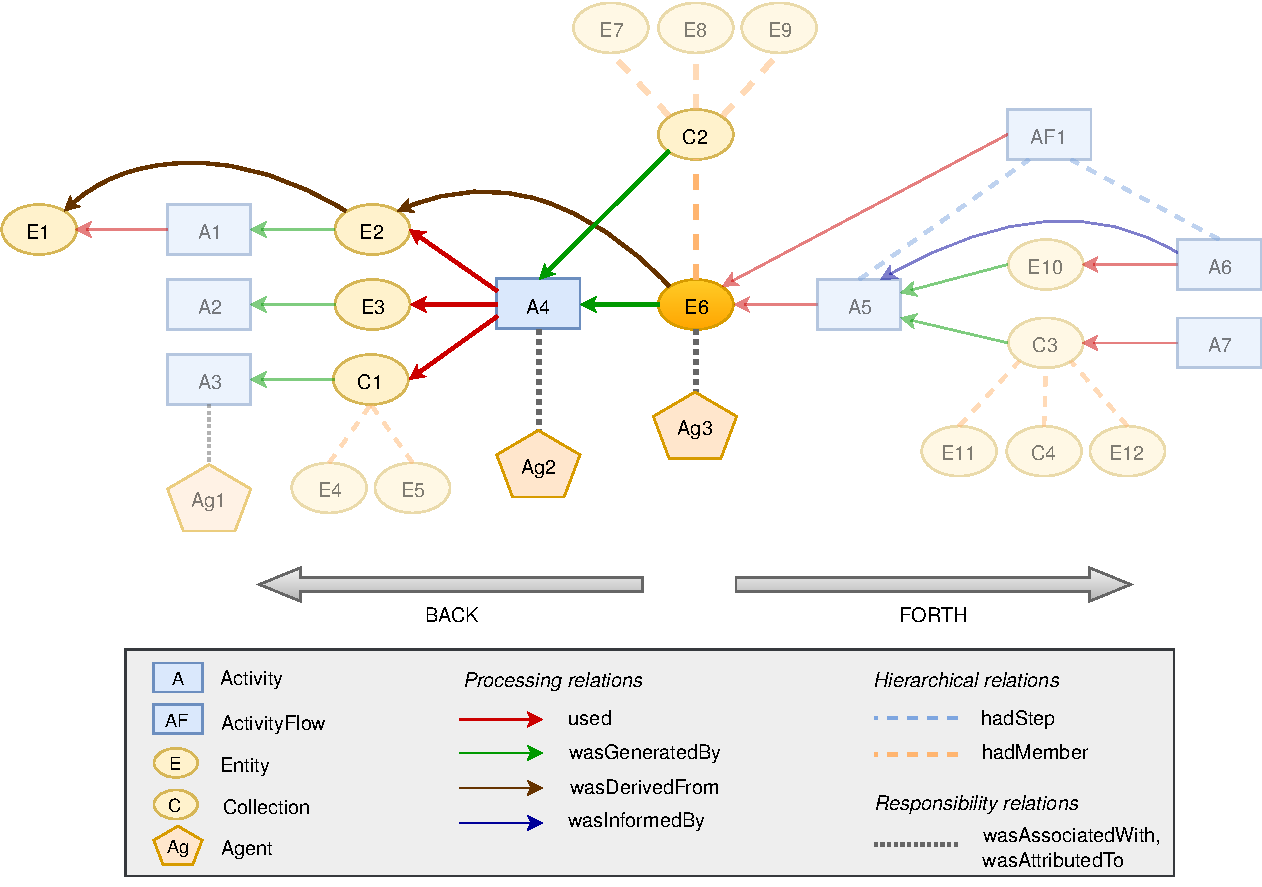
\includegraphics[width=1.0\textwidth]{provenance-graph-example-depth2.pdf}
\caption{An example provenance graph, highlighting the objects and relations returned from a ProvDAL service with \texttt{ID=E6} and \texttt{DEPTH=2}. The BACK and FORTH values for DIRECTION are only important for the processing relations (solid lines). Hierarchial (dashed) and responsibility (dotted) relations are only followed ``upwards'' (to collection/activityFlow) and towards agents by default (unless the optional parameters MEMBERS, STEPS and/or AGENT are set to true.}
\label{fig:provenance-graph-example}
\end{figure}




\paragraph{MEMBERS, STEPS}
The provenance data model defines the hierarchical relations \emph{hadMember} for entity collections and \emph{hadStep} for activityFlows. If a node belongs to a collection or activityFlow, these relations shall be returned as well, independent of the specified tracking direction.
If someone is interested in more details and wants to follow the \emph{members} of an entity collection or the \emph{steps} of an activityFlow, these can be included by setting the optional parameter MEMBERS or STEPS to true, respectively. The default is false. As detailed in DALI, the values 1 and 0 are equivalent to true and false.

\paragraph{AGENT}
By default, it is recommended to stop any further tracking at an agent node, unless an additional optional parameter AGENT is set to true. Note that this means that the request for any agent will always return just the agent node itself and nothing else, unless AGENT=true is used. An example request if one wants to know which entities and activities an agent has influenced could look like this:\\\texttt{\{provdal-base-url\}?ID=org:rave\&AGENT=true\&DEPTH=1}.\\
\texttt{DEPTH=1} is used here in order to avoid following the found entities and activities any further (can be omitted, since this is the default for DEPTH).
\newline
%\comment{Maybe it's better to use DEPTH and DIRECTION instead of FORWARD and BACKWARD. Reason: if a service just implements the backward direction, then it's weird to call something ``backward'' if there is no ``forward'' as well. DEPTH is also a commonly used word when refering to graphs and numbers of relations.}



A ProvDAL service MUST implement the parameters ID, DEPTH and FORMAT; the remaining parameters are optional.
If a service does not implement the optional parameters, but they appear in the request, then the service should return with an error.
Please note that according to the DALI specification \citep{std:DALI}, the parameter names are case-insensitive, but the parameter values are not. E.g. \texttt{direcion=FORTH} is allowed, but \texttt{DIRECTION=forth} may not work.


\subsubsection{ProvDAL example use cases}
We provide here a few example use cases for ProvDAL in order to show its usefulness in exploring the provenance
of astronomical datasets, processes or the people and projects involved in producing/performing them.

\begin{itemize}
\item The RAVE DR4 release contains a main table with stellar properties for each observation of a star. Given the RAVE observation ID, retrieve the processing steps
for this specific observation result:

	\begin{verbatim}
	{provdal-base-url}?ID=rave:20121220_0752m38_089&DEPTH=ALL
	\end{verbatim}

The result will not only contain the processing steps (activities), but also entities and agents. The important information can be filtered out by a client application (e.g. use voprov Python package). If a W3C tool shall be used, one needs to transform the response into a W3C compliant serialisation (e.g. for loading the result to ProvStore\footnote{https://provenance.ecs.soton.ac.uk/store/} for further processing).

\item Get the direct progenitor of an entity:
	\begin{verbatim}
	{provdal-base-url}?ID=rave:20121220_0752m38_089&DEPTH=1
	\end{verbatim}
	If this request only returns a collection and not any ``backwards'' information about progenitors, then
	one needs to track the collection further, i.e. repeat the request for the collection entity.

\item Get all datasets that were derived from a specific data file in the CTA pipeline:
	\begin{verbatim}
	{provdal-base-url}?ID=cta:df1&DEPTH=ALL&DIRECTION=FORTH
	\end{verbatim}
	By using \texttt{DIRECTION=FORTH} we can track the dataset and where it was used forward.

\item Find all people that were involved in processing a dataset along with their contact data (if available), so that one can ask them for further information.
	\begin{verbatim}
	{provdal-base-url}?ID=ex:e1&DEPTH=ALL
	\end{verbatim}
 	The ProvDAL request is basically the same as in the first example. From the results the agents need to be filtered.
 	Since the response contains the nodes and relations including all their properties, the contact details for the agents are included as well (if they are stored with the service).

\item Retrieve a VOTABLE serialisation of the provenance for an image from a data collection.
	\begin{verbatim}
	{provdal-base-url}?ID=myproject:img1&DEPTH=ALL&FORMAT=PROV-VOTABLE
	\end{verbatim}
	We use the FORMAT keyword here to retrieve a VOTABLE.
\end{itemize}

ProvDAL is meant to be used to retrieve parts of a provenance graph from a provenance web service. It cannot be used to retrieve information based on specific properties, e.g. the creationTime of an entity or a parameter value for an activity. For such cases, a ProvTAP service can be used (see next section).


\TODO{Add paragraph on VOSI-endpoints? (DALI service!)}



\subsection{ProvTAP}
ProvTAP is a TAP service implementing the ProvenanceDM data model. The data model mapping is included in the TAP schema. The mapping of ProvenanceDM classes and attributes onto tables and columns of the schema with the appropriate relationships, datatypes, units, utypes and ucds is done similarly to the PROV-VOTABLE serialization. The query response will result in a single table according to the query.
This single table is joining information coming from one or several ``provenance'' tables available in the database.

A special case is considered where ProvenanceDM and ObsCore are both implemented in the same TAP service and queried together. The TAP response is then providing an Obscore table with a ProvenanceDM extension. We can imagine that in the future this could be hard-coded and registered as an ObsProvTAP service.


\TODO{We need more details here! Output of TAP service is NOT a PROV-VOTABLE by default!}

%\TODO{Do we need combined query possibilities, i.e. ask for ObsCore-fields and Provenance fields in one query? Or rather use a 2-step-process, decoupling them from each other?}


%\TODO{Also look at PROV-AQ from the W3C.}

\subsection{VOSI availability and capabilities}
According to the DALI specification for VO services \citep{std:DALI}, a provenance service implementing ProvDAL and/or ProvTAP must provide a VOSI availability interface as well as a capabilities interface with entries for ProvDAL and/or ProvTAP. The \texttt{standardId}s for these provenance interfaces are:

\begin{verbatim}
ivo://ivoa.net/std/ProvenanceDM#ProvDAL-1.0
ivo://ivoa.net/std/ProvenanceDM#ProvTAP-1.0
\end{verbatim}

The capability for a TAP service to support the Provenance DM is expressed by the dataModel element as :
\begin{verbatim}
<dataModel ivoid="ivo://ivoa.net/std/ProvenanceDM#core-1.0">ProvenanceDM-1.0</dataModel>
\end{verbatim}

For ProvTAP, the VOSI tables interface also needs to be provided.




\section{Discussion}
\section{Discussion}

\subsection{Links, ids}\label{sec:links_between_data}
It would be convenient, if each data object or even each file 
gets a unique id that can be referenced. The W3C provenance model requires ids
for entities, activities and agents, and they have to be qualified strings, 
i.e. containing a namespace. For example, an activity in the RAVE-pipeline could 
have the id `\texttt{rave:radialvelocity\_pipeline\_20160901}'. Using a namespace for each 
project for these ids will help to make them unique. 

If several copies of a dataset exist, and one of them is corrupted, it would even be useful to know
exactly which copy was used by a given activity. This can be modeled already 
with the existing tools (using a copy-activity), but we doubt that many people
would actually need this level of detail.

IVOIDs and DOI's are potentially good candidates for unique identifiers.


%\subsubsection{Calibration data}
%The calibration dataset consists of images that can be used to calibrate the
%raw data. It is not necessary to mention them explicitly in the model, 
%they are just another dataset that is used by activities with a 
%calibration-method.

%\subsubsection{Quality}
%For expressing the quality of data, we could simply define additional 
%attributes for each \class{Activity}
%or \class{Entity} object, i.e. zero, one, or more properties in the form of
%key-value pairs. We could use a \class{Quality} namespace to mark a keyword
%as quality-related:
%\begin{itemize}
%    \item quality:comment: [some text]
%    \item quality:seeing: [some value]
%\end{itemize}
%The values could range from a float number to free text.


%\subsubsection{Provenance of provenance}
%``Bundles'' are used to name a set of provenance descriptions. It is a type for 
%an entity, and allows to express provenance of provenance. This is probably  
%very interesting for workflow systems.
% -- partially covered already with ActivityFlow

\subsection{Discussion of description side}
This model was established mainly having a database implementation in mind. 
However, it may be better in the long run to store provenance with 
the entities themselves, e.g. as an additional extension in fits-headers.

A model using a description side for defining templates for activities and
entities has an advantage for normalization: the common processes could be 
described once and for all at some place and then be reused when recording
provenance information for certain entities and activities. This \emph{some place} 
is actually the crucial point here.
In an ideal world, ``some place'' could collect all the descriptions from all 
the possible datasets and methods in astronomy, but building such a look-up place 
is a quite challenging task -- it will probably never be complete. There's also 
the issue of persistent identifiers/broken links to consider.
Normalisation is useful for closed systems, e.g. for describing the provenance 
for data produced by a certain pipeline (e.g. MuseWise system) or with 
workflow tools or when a task needs to be repeated many times. However, the VO 
is quite the contrary of a closed system and we need to keep an eye on what is 
actually achievable.

When writing down a simple serialisation of e.g. the provenance for a stacked 
image using the current model including the description classes, it soon becomes quite cumbersome to define 
everything twice: first the descriptions, then the instances. This basically 
doubles the number of entries to describe provenance (unless there is already 
some place with all the descriptions to which we can refer).

Expressing provenance for a stacked image with this smaller set of classes may 
be simpler, but on the other hand constructing a database schema becomes much 
harder. 
We could leave it to the implementors to choose what is more useful for them.
When extracting a serialisation of the provenance information from a provenance 
service, the attributes of the description classes could be combined with 
the corresponding activity/entity classes. This will produce some repetition
(e.g. many entities may have the same descriptive attributes), but 
avoid having too many classes and links between them.
% Note: Harry Enke commented that this sentence is not understandable; 
% we can remove this sentence later on when we have a proper implementation-note section.
%\Note{Descriptions could be present in W3C-conform serialisations, if we 
%put them into entities.}

%\TODO{Check, if PROV-Templates from the W3C (inofficial note) could be used 
%for ActivityDescriptions.}

\subsection{Discussion of ActivityFlow}
By introducing the \class{ActivityFlow} class, one entity can now have many 
wasGeneratedBy-links to activities. One of them would be the actual generation-activity, 
the other activities can only be activityflows containing this generation-activity.
This is not expressed explicitly in the current model. 

We could introduce an additional abstract class, e.g. \class{AbstractActivity}, with \class{Activity} and 
\class{ActivityFlow} being subclasses to this one. But this adds another layer of complexity 
that we may not want in this data model.

Since we introduced \class{ActivityFlow} mainly for having different view levels, 
we may want to add an attribute \emph{viewLevel} to descriptions of activityflows.

We are planning to test how it all works in implementations, which classes and attributes are 
needed or not and will then adjust the model 
accordingly.

\subsection{VO-DML representation}
We do not yet have a VO-DML compliant representation of the model. This is one 
of the issues to be clarified for the next version.

\subsection{Links to other data models}
Section~\ref{sec:dmlinks} still needs to be expanded further, especially making detailed links with the 
Simulation Data Model will be very useful.



\section{Implementations of the data model for specific use cases}
\label{sec:usecases-implementations}
%\subsection{One processing step in PROV-N notation}
%
%\TODO{Put the very simple example here}
%See \url{https://volute.g-vo.org/svn/trunk/projects/dm/provenance/description/prov-example-incl-prototypes.txt}
%and \url{https://volute.g-vo.org/svn/trunk/projects/dm/provenance/description/prov-example-w3c.txt}

This section presents some general guidelines for applying the data model and
%This section presents some 
specific use cases for which the provenance data model helps to solve certain tasks. Details on specific implementions of the provenance data model are provided in a separate document, the ProvenanceDM Implementation Note \citep{std:ProvenanceImplementationNote}.


\subsection{How to use the data model}
%\TODO{KR: I think this is a good place for this section. Do we still want to have this section or is everything covered with the new section on entitydescription-serialisation?}
%\begin{itemize}
%\item identify entities in your project, i.e. the things you deal with
%\item identify activities (processes) in your project
%\item identify reponsible agents (persons and organizations)
%\item find the relations between them
%\item possibly disentangle entity properties and entityDescription properties: everything that you may know about an entity before its creation, belongs to the entityDescription; e.g. file format, dataProduct\_type, what kind of entity it is going to be (category)
%\item ...
%\end{itemize}

The IVOA Provenance data model has been developed along with its implementations into different projects. We gather here some tips to apply the model to a specific project.

\paragraph{Before using the model}
We noticed that the simple knowledge of what is provenance information is important for the development of all projects. Before using or not the Provenance data model and associated services, it is good practice to locate and collect information on activities, entities and agents, and be sure that this information is not lost along the way. For example, a script may use intermediate files (such as calibration files for observations) that may not be tracked by the system.

\paragraph{Define unique identifiers}
It would be convenient, if each data object or even each file 
gets a unique id that can be referenced. The W3C provenance model requires ids
for entities, activities and agents, and they have to be qualified strings, 
i.e. containing a namespace. For example, an activity in the RAVE-pipeline could 
have the id `\texttt{rave:radialvelocity\_pipeline\_20160901}'. Using a namespace for each 
project for these ids will help to make them unique. 
IVOIDs, DOI's or ORCIDs are potentially good candidates for unique identifiers.

\paragraph{Use of the description classes} 
One may only use the core data model without the description classes if they are not needed for the project. In that case, it is recommended to include the attributes of the description classes into the main classes (Entity/Activity/Agent, and if needed Parameter). In the same way, when serializing the provenance information, the description classes can be merged to the main classes, which is needed to produce W3C compliant provenance files.

\paragraph{Identify entities, activities and agents}
If inside the project, the different entities are already identified, as well as the activities producing them, then the description classes are probably of interest and will help to reduce the redundancy in the provenance information stored.

\paragraph{Add project specific attributes to entities, activities and agents}
We proposed generic attribute for the different classes, but there are probably project specific attributes that need to be added. 
It is also required at this level to disentangle entity properties and entityDescription properties: everything that you may know about an entity before its creation, belongs to the entityDescription (e.g. file format, dataProduct\_type, category).

\paragraph{Create ActivityDescription files}
A model using description classes for defining templates for activities and
entities has an advantage for normalization: the common processes could be
described once and for all at some place and then be reused when recording
provenance information for certain entities and activities.
If description classes are relevant for a projet, it may be sufficient to store the descriptions directly as ActivityDescription files (see Section \ref{sec:description-serialization}). 
Those can be created and centralized before implementing a provenance database or service.

\paragraph{Link to an Authentication System}
We proposed to add optional attributes to tha Agent class (email, phone, address). However, a project may already include an authentication system with a user directory. In that case the Agent identifiers should be the ones used in the authentication system.

\paragraph{Adding additional metadata to an existing Entity}
It could happen that after creating entities and storing their provenance, additional metadata is needed for those entities. For example, an ObsCore description may have to be added to some entities when they are made available to the public. In that case, the entity will receive an external identifier (e.g. a publisher\_did), which should thus be associated to the entity provenance identifier (Entity.id) in a relation table.


\subsection{voprov Python package}\label{sec:implementation_voprov}
The voprov Python package is derived from the voprov-package. It can load
data and serialize it. The voprov-package supports following features:
...
\TODO{Michele: Please add more explanations!}
%This code writes the serialisation examples which are given in Section~\ref{sec:serialisations}.

Example code and serializations are given in the Implementation Note \citep{std:ProvenanceImplementationNote}.


\subsubsection{Graphic formats}
\label{sec:graphic_formats}
The voprov python module can also provide provenance information in graphic formats: PNG, SVG and PDF.
In the above example, you have to add the following instructions in your python program:

\begin{verbatim}
    dot = prov_to_dot(provdoc, use_labels=True)
    dot.write_png('ex1.png')
    dot.write_svg('ex1.svg')
    dot.write_pdf('ex1.pdf')
\end{verbatim}

\begin{figure}
\centering
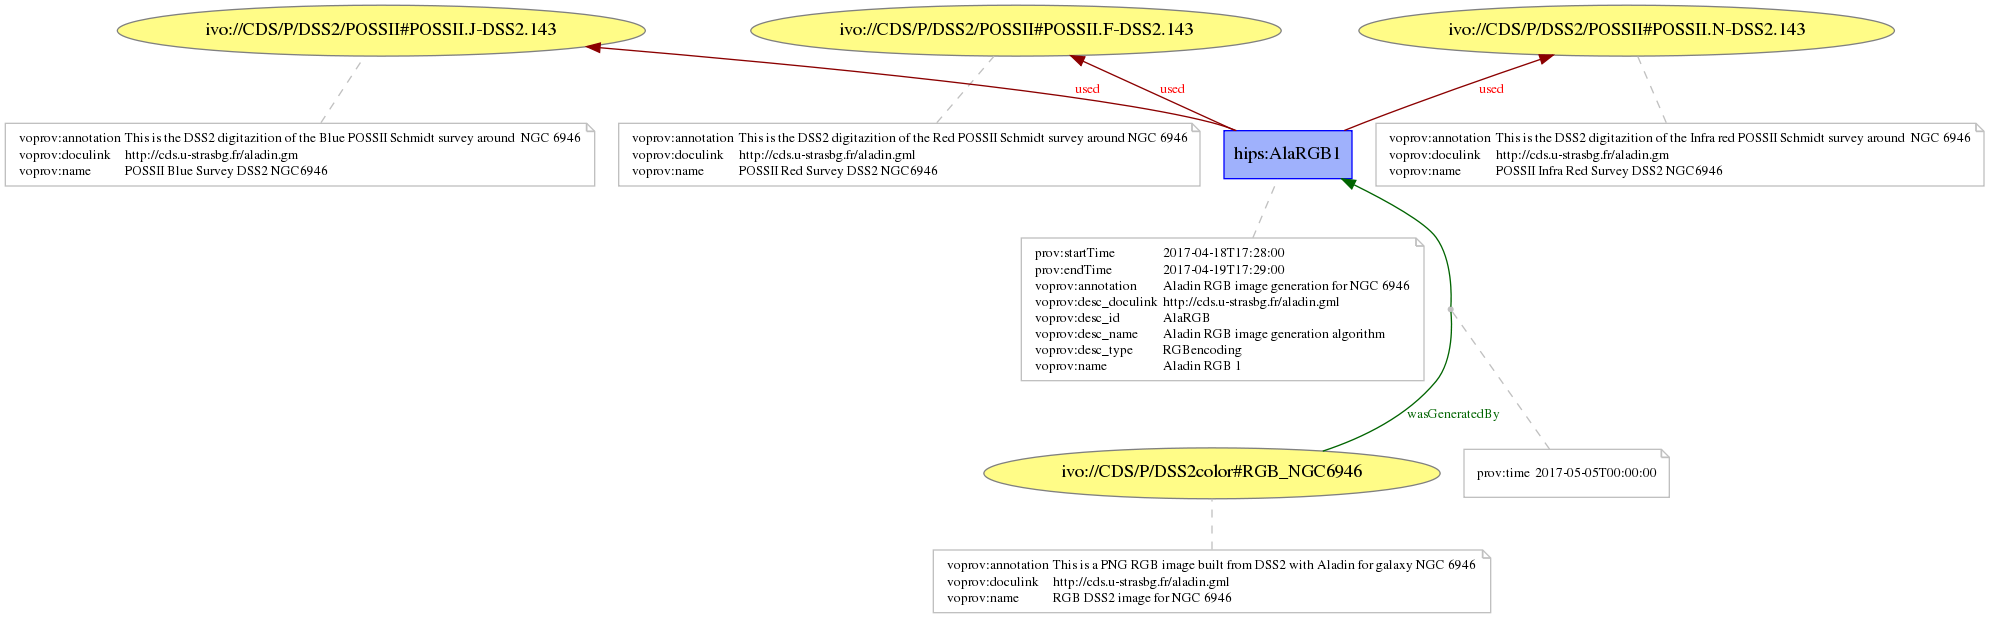
\includegraphics[width=0.9\textwidth]{access_ex1.png}
\caption{Example: png format@}
\label{fig:example}
\end{figure}



\subsection{Provenance of RAVE database tables (DR4)}
The RAVE survey (Radial Velocity Experiment) recorded spectra for about half a 
million stars. These spectra are processed in a number of steps until the 
derived properties are published in the RAVE data releases at http://www.rave-survey.org.
Providing provenance information for the data, from which spectrum and fibre the
data was coming from and which steps were involved in processing the data, can help scientists
to understand the data and their restrictions and judge their quality.
It would also be useful to be able to compare if, how and why the derived data 
for some stars have changed between different releases.
Provenance information for some major steps of RAVE DR4 was loaded in 
W3C-compatible PROV-N notation and uploaded to the provenance store at 
https://provenance.ecs.soton.ac.uk/store/documents/84064/. This allows to view 
graphs of the workflow by visualising only the main entities, activities and agents 
with their relations. It shows that the provenance concepts explained in this draft 
can be applied directly to data obtained from astronomical observations.

We also tested a Django implementation of the classes in this document along with provenance data stored in an SQLite database. This allows to quickly setup a provenance web service
which gives the possibility to view all instances of a class or details for a single object, 
extract provenance information for single entities (backwards in time) and 
visualise the provenance information. 
More details about this are available in the implementation notes \citep{std:ProvenanceImplementationNote}.




\subsection{Provenance for CTA}

The Cherenkov Telescope Array (CTA) is the next generation ground-based very high energy gamma-ray instrument. It will provide a deep insight into the non-thermal high-energy universe. Contrary to previous Cherenkov experiments, it will serve as an open observatory providing data to a wide astrophysics community, with the requirement to propose self-described data products to users that may be unaware of the Cherenkov astronomy specificities. The proposed structure of the metadata is presented in Figure~\ref{fig:cta_dm}.

\begin{figure}
\centering
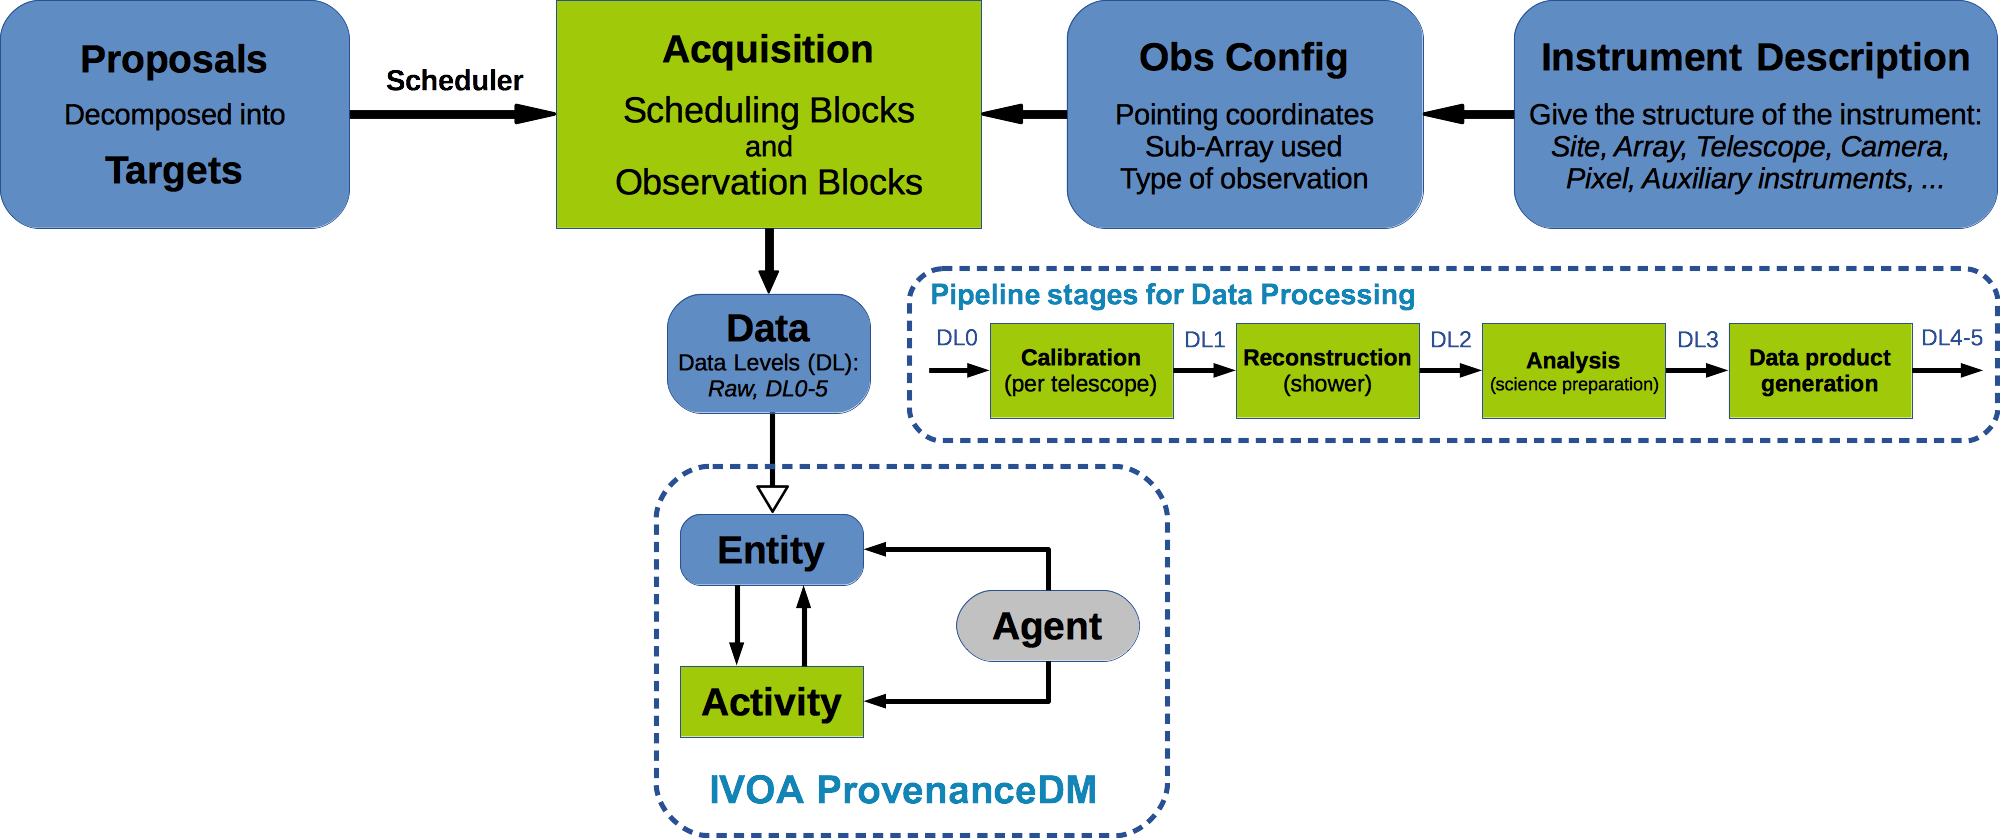
\includegraphics[width=\textwidth]{CTA_DM_high_level.png}
\caption{CTA high level data model structure with Pipeline stages and connection to IVOA ProvenanceDM.}
\label{fig:cta_dm}
\end{figure}

Cherenkov telescopes indirectly detect gamma-rays by observing the flashes of Cherenkov light emitted by particle cascades initiated when the gamma-rays interact with nuclei in the atmosphere. The main difficulty  is that charged cosmic rays also produce such cascades in the atmosphere, which represent an enormous background compared to genuine gamma-ray-induced cascades. Monte Carlo simulations of the shower development and Cherenkov light emission and detection, corresponding to many different observing conditions, are used to model the response of the detectors.  With an array of such detectors the shower is observed  from several points and, working backwards, one can figure out the origin, energy and time of the incident particle. The main stages of the CTA Pipeline are presented inside Figure~\ref{fig:cta_dm}. Because of this complexity in the detection process, provenance information of data products is necessary to the user to perform a correct scientific analysis.

Provenance concepts are relevant for different aspects of CTA :
\begin{itemize}
\item Data diffusion: the diffused data products have to contain all the relevant context information with the assumptions made as well as a description of the methods and algorithms used during the data processing.
\item Pipeline: the CTA Observatory must ensure that data processing is traceable and reproducible.
\item Instrument Configuration: the characteristics of the instrument at a given time have to be available and traceable (hardware changes, measurements of e.g. a reflectivity curve of a mirror, ...)
\end{itemize}

We tested the tracking of Provenance information during the data analysis using the Python prov package inside OPUS\footnote{\url{https://github.com/ParisAstronomicalDataCentre/OPUS}} (Observatoire de Paris UWS System), a job control system developed at PADC (Paris Astronomical Data Centre). This system has been used to run CTA analysis tools and provides a description of the Provenance in the PROV-XML or PROV-JSON serialisations, as well as a graph visualization (see Figure~\ref{fig:cta_prov}).

\begin{figure}
\centering
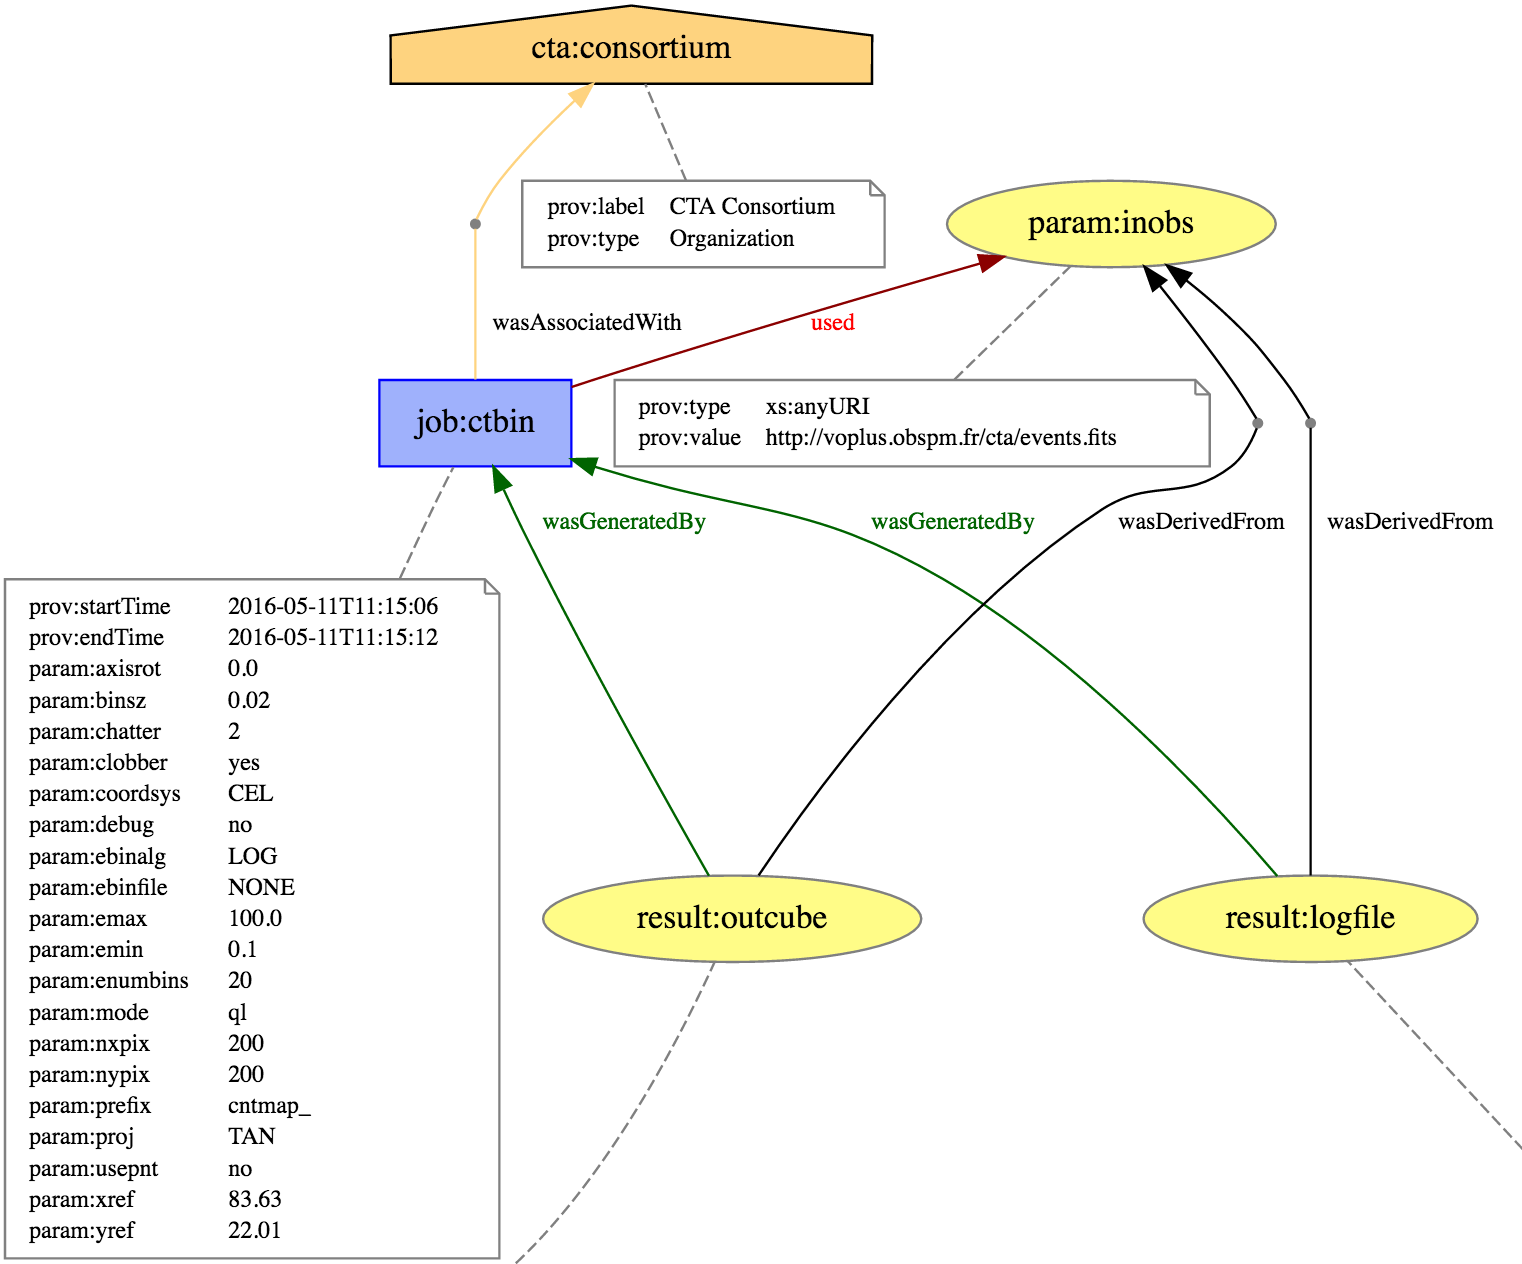
\includegraphics[width=0.8\textwidth]{CTA_prov.png}
\caption{Provenance description of a CTA analysis step.}
\label{fig:cta_prov}
\end{figure}

The CTA Pipeline contains a specific Provenance class dedicated to the collection of provenance information after each processing step. This informations is returned as an output file for now.

More details about the related implementations are available in the implementation notes \citep{std:ProvenanceImplementationNote}.


\subsection{Provenance for the POLLUX database}

POLLUX is a stellar spectra database proposing access to high resolution synthetic spectra computed using the best available models of atmosphere (CMFGEN, ATLAS and MARCS), performant spectral synthesis codes (CMF\_FLUX,SYNSPEC and TURBOSPECTRUM) and atomic linelists from VALD database and specific molecular linelists for cool stars. 

Currently the provenance information is given to the astronomer in the header of the spectra files (depending on the format: FITS, ascii, xml, votables, ...) but in a non normalized description format. 

The implementation of the provenance concepts in a standardized format allows users on one hand to benefit from tools to create, visualize and transform in another format the description of the provenance of these spectra and on a second hand to select data depending on provenance criteria.

\begin{figure}
\centering
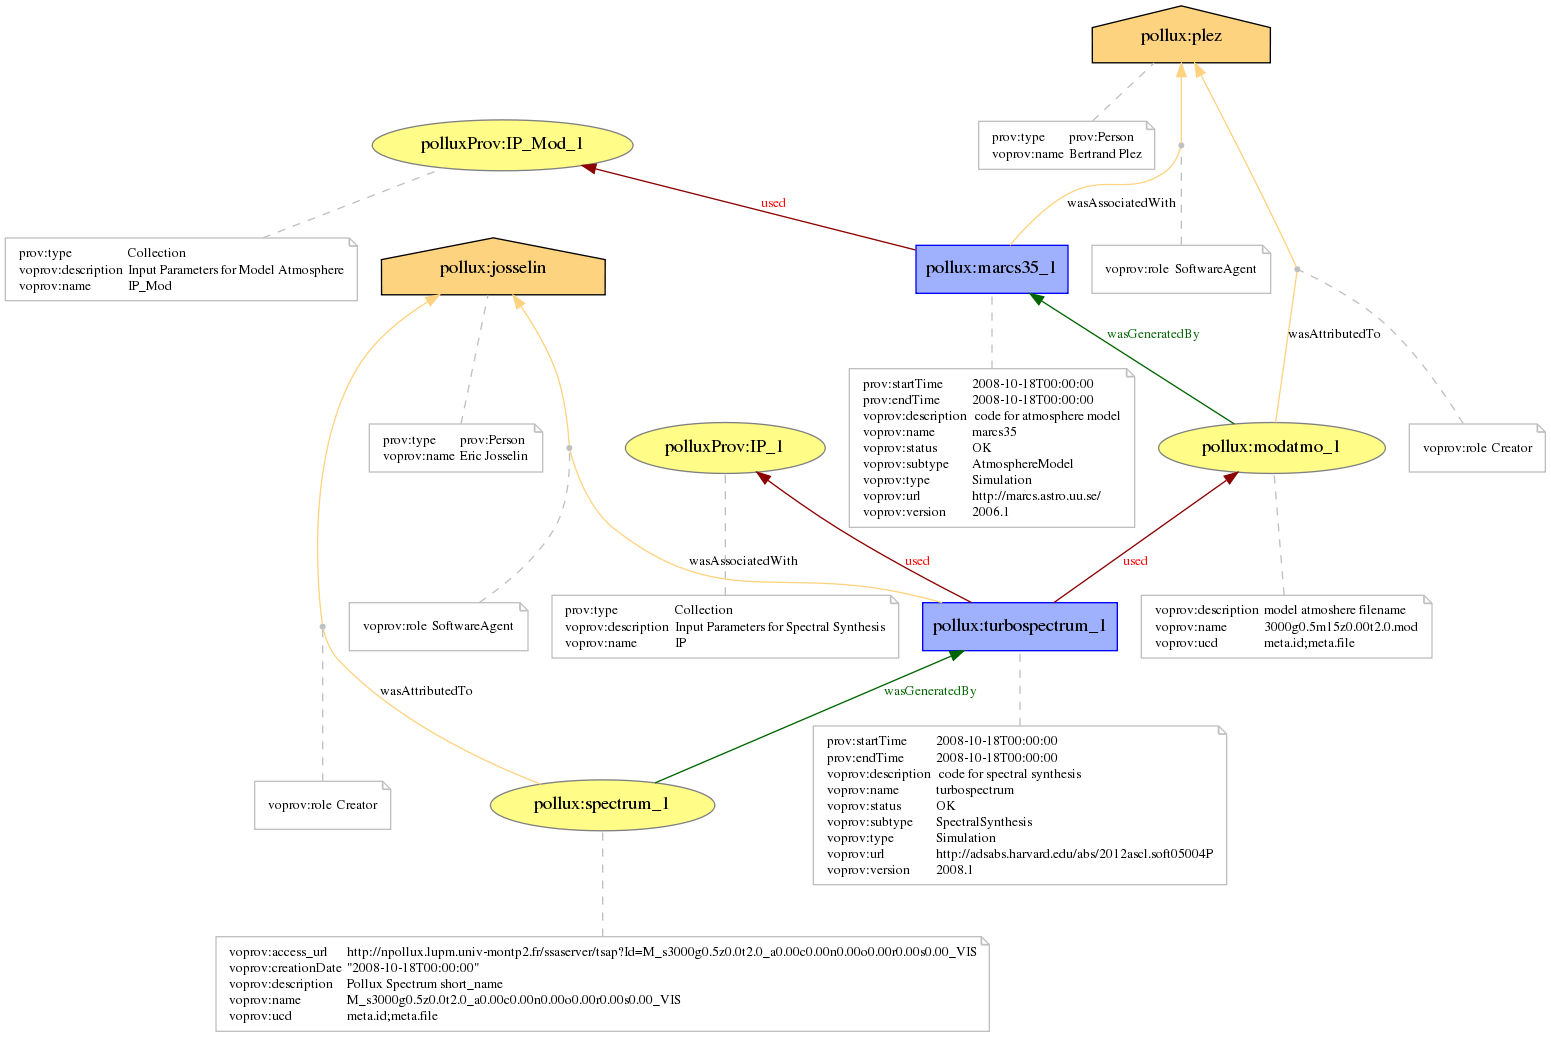
\includegraphics[width=0.9\textwidth]{usecase_Pollux_example1.png}
\caption{Pollux Example 1}
\label{fig:pollux}
\end{figure}

\subsection{Provenance of HiPS datasets}
HiPS is a new all sky organization of pixel data. It is based on HealPix tesselation of the sky on equal area cells (pixels) for a given HealPix order gathered in tiles. Adaptative resolution is achieved by a hierarchy of tiles at increasing order. Sorting and organization is based on a tree of including directories each of those associated with a tile. HiPS specification has entered the IVOA recommendation process and is becoming an interoperability standard.
In the processing chain, HiPS can be seen as a kind of ``legacy level'' for observational data.


An HiPS dataset can be generated either by Aladin in ``hipsgen'' mode or by other softwares \cite{if others}.  The processing distinguishes 3 main different methods for estimating cell values with parameters: FIRST(nearest neighbour), MEAN and MEDIAN of the neighboring pixels. Up to 50 parameters can help to tune the processing, among which the higher resolution HealPix order, the sky background value to be substracted, the border width or the mask to apply to original images to avoid including bad area in the computing, etc.


An example of provenance metadata for a HiPS collection generated from a collection of SERC Schmidt plates scanned by CAI-Observatoire de Paris with the MAMA facility and serialized in PROV-N format is given at 
\url{https://volute.g-vo.org/svn/trunk/projects/dm/provenance/example/HiPS-prov-provn.txt}, the corresponding votable-format is available at \url{https://volute.g-vo.org/svn/trunk/projects/dm/provenance/example/HiPS-prov-vot.xml}.

Here is an excerpt of the corresponding PROV-N serialization:

\begin{verbnobox}[\scriptsize]
Entity
( ivo://CDS/P/MAMA/ESO-R, 
[ voprov:name = "ESO-R MAMA HIPS at CDS",
voprov:annotation = "This is the HiPS version of ESO Schmidt survey digitized by Mama and processed by CDS",
voprov:type= "voprov:entity",
voprov:access_reference = "http://CDS/P/MAMA/ESO-R", // as defined in obscore 
voprov:doculink = "http://cds.u-strasbg.fr/hips/documentation.html#structure",
voprov:level = 3,
hips:dataproduct_type = "voprov:hips_pixels",
hips:HiPS_properties = "http://cds.u-strasbg.fr/hips/p/mama/eso-r/properties.txt"] )

// Relationship
WasAttributedTo(ivo://CDS/P/MAMA/ESO-R,  ivo://cds, prov:role= "voprov:creator")

Agent
(ivo://cds,
[ voprov:Name= "CDS",
voprov:contact = "question@astro.unistra.fr",
voprov:type = "Organisation" ]) 

WasGeneratedBy  (ivo://CDS/P/MAMA/ESO-R, EHG1, -) 

Activity
(EHG1,
[ voprov:name = "ESO HiPS generation 1",
voprov:startTime = "2016-07-18", 
voprov:endTime = "2016-07-20",
voprov:annotation = "This activity is final generation of HiPS for ESO Mama survey",
voprov:activityDescription = "HipsgenM"] )
 
ActivityDescription 
(HipsgenM,
[ voprov:name = "HiPSgen_Mean",
voprov:type = "data encoding",
voprov:subtype= "HiPSgen_MEAN",
voprov:doculink = "http://cds.u-strasbg.fr/HiPSGEN-Documentation"])

WasAssociatedWith( EHG1, Buga, voprov:role="voprov:operator")
WasAssociatedWith(EHG1, ivo://CDS, prov:role="voprov:creator")
WasAttributedTo(( ivo://CDS/P/MAMA/ESO-R, buga, prov:role= "voprov:operator")
\end{verbnobox}



\appendix
\section{Changes from Previous Versions}
\subsection{Changes from WD-ProvenanceDM-1.0-20161121}
\begin{itemize}
\item rights instead of access in Entity class 
\item parameter example tables 
\item pollux figure size . not yet changed  
\end{itemize}
% No previous versions yet.
% these would be subsections "Changes from v. WD-..."
% Use itemize environments.
\subsection{Changes from WD-ProvenanceDM-1.0-20161121}
\begin{itemize}
\item Moved detailed implementation section from appendix to a separate document (implementation note)
\item Removed description\_ref as attribute, since it's expressed by the corresponding link in the model anyway.
\item More explanations on links to data models in Section~\ref{sec:dmlinks}.
\item Introduced subsections for Section~\ref{sec:dmlinks}, added table with SimDM-links.
\item Renamed \emph{docuLink} to \emph{doculink}
\item Avoid double-meaning of \emph{description} by splitting it up into: 
    \begin{itemize}
    \item \emph{description\_ref}: a foreign key, reference to a description class 
(which could be located at an url as well)
    \item \emph{annotation}: free text description
    \end{itemize}
\item Applied similar naming scheme to \emph{Parameter} and \emph{ParameterDescription}-classes
\item Renamed \emph{Agent.name} to \emph{Agent.label}, so that each class has an id and a label.
\item Renamed Section~\ref{sec:usecases-implementations} to stress that it deals with implementations.
\item Added links to provn and votable-serialization for HiPS-use case, added first part of provn as example in the HiPS-use case section.
\item Corrected attribute names in Table~\ref{tab:datasetmapping}.

\end{itemize}


% \section{Implementation details}\label{sec:implementation-details}
% In this section we will give more details on the classes and attributes which were used 
% in implementations for each use case. This maybe needs to go into a different document, so it can 
% be updated without affecting this standard.

% TBD.


\bibliography{ivoatex/ivoabib,prov-refs}


\end{document}
